This chapter considers the case of linear constraints.   Specifically,  we present several variants of a trust region method for solving the problem 

\sbnote{Change the following to $Ax \le b$}
\begin{equation} \label{eq:DFO-linear}
\begin{array}{ccl} \min_{x \in \Rn} & f(x) \\
& Gx \le g, & 
\end{array}
\end{equation}
where $f:\Rn\rightarrow\reals$ is a black-box function,  $G$ is an $m \times n$ matrix and $g \in \Rm$.

To define our methods, we distinguish between two types of trust regions:  a {\em sample trust region}, $\sampletrk$, from which the sample points are chosen,  and a {\em search trust region}, $\searchtrk$, which is the feasible region for the trust region subproblem.     For unconstrained optimization,  these trust regions are typically identical,  and are chosen to be an $L_2$-ball of radius $\Delta_k$.    However, for constrained optimization, it is useful to distinguish between the two regions.  

Both of these trust regions will be required to lie within the feasible region $\feasible := \{x|Gx \le g\}$, and also to lie within an  {\em outer trust region}, $\outertrk = B_1(x^{(k)},\Delta_k)$,  which is an $L_{\infty}$-ball of radius $\Delta_k$ centered at the current iterate $x^{(k)}$.     

We consider two main strategies for defining these trust regions.
In the first method,  which is described in \cref{sec:ellipsoidal},  we define $\sampletrk$ to be an ellipsoidal region that lies within the intersection of the feasible region and the outer trust region.    This is referred to as the {\em ellipsoidal trust region approach}.    The advantage of this approach is that it is relatively straightforward to modify the model-improvement algorithm \cref{model_improvement} to construct a well-poised sample set over an ellipsoidal region.    In this method, we define the search trust region by  $\searchtrk=\outertrk \cap \feasible$.   Note that by using an $L_{\infty}$-ball instead of an $L_2$-ball, the search trust region is a bounded polyhedron,  which makes the trust region subproblem a quadratic program.  \sbnote{Maybe make a comment somewhere about why we are not using the ellipsoid as the search trust region.}

In the second method,  described in \cref{sec:polyhedral}, we define \[\sampletrk = \searchtrk = \outertrk \cap \feasible.\]
Since this trust region is a bounded polyhedron,  we call this the {\em polyhedral trust region approach}.
While this method is perhaps more intuitive than the first approach, it is not immediately clear how to construct a well-poised sample set over the polyhedral region.  We present one method for doing this.   \sbnote{Come back to the wording of this.}

In all cases, the trust regions are related by the inclusions
\[\sampletrk \subseteq \searchtrk \subseteq \outertrk \cap \feasible
\]
Both methods fall into a general algorithmic framework, which we describe next.

We consider two main strategies for defining the sample trust region.
In the first method,  which is described in \cref{sec:ellipsoidal},  we define $\sampletrk$ to be an ellipsoidal region that lies within the intersection of the feasible region and the outer trust region.    This is referred to as the {\em ellipsoidal trust region approach}.     For this approach, we present a method for selecting a well-poised set of sample points by a straightforward application of the model-improvement algorithm \cref{model_improvement} to a transformed problem in which the ellipsoidal region is mapped onto a ball.

The second method, which is described in \cref{sec:polyhedral} defines the sample trust region by $\sampletrk = \outertrk \cap \feasible$.  
Observe that by using an $L_{\infty}$-ball instead of an $L_2$-ball, the trust regions are polytopes.
We therefore call this the {\em polyhedral trust region approach}.
To select sample points from this polyhedral region, we present a modification of model-improvement algorithm \cref{model_improvement}.


We also consider two strategies for defining the search region.
The

\section{Algorithm Template}\label{sec:template}
All of the methods in this chapter follow
an algorithmic template described in \cite{doi:10.1080/10556788.2015.1026968}, 
\sbnote{check this reference--I suspect it might be \cite{conejo.karas.ea:global} instead--if it is, then maybe also add ``which describes a class of trust-region algorithms for convex constrained minimization without derivatives. '' 
}.   Different variations of the algorithm have different choices of $ \sampletrk $ implemented in a \emph{ConstructTrustRegion} subroutine.
The different versions are described in the remainder of this chapter.

% HOW ABOUT JUST MAKE $\eta > 0$?

\sbnote{Check this algorithm carefully}

  \sbnote{$sk$ should be $\argmin$, not $\min$ in Step 3 of the algorithm}
  
  \sbnote{$\chik$ versus $\chi_k$?}
  
  \sbnote{Should last bullet of Step 4 have $\Delta_{k+1} = \min( \omegainc\dk, \Delta_{\text{max}})$?}

\begin{algorithm}[H]
    \caption{Simplified Always-feasible Constrained Derivative Free Algorithm}
    \label{linearly_constrained_dfo_simple}
    \begin{itemize}
        \item[\textbf{Step 0}] \textbf{(Initialization)} \\
            Choose parameters
            $\tolcrit\ge 0$,$\tolrad \ge 0$, $\omegadec \in (0,1)$, $\omegainc \ge 1$,  
            $ \gammabi \in (0,1]$, $\gammasm \in (0,\gammabi)$, and $\alpha > 0$.   Choose starting 
            point $x^{(0)} \in \feasible$ and $\Delta_0 > 0$. and set $k\gets 0$.
            
        \item[\textbf{Step 1}] \textbf{(Construct the model)} \\
           Construct the trust regions $\sampletrk$ and $\searchtrk$.  Select sample points within $\sampletrk$,  and construct the model function $\mfk$.       
        
        \item[\textbf{Step 2}] \textbf{(Check stopping criteria)} \\
            Compute the criticality measure $\chi_k$.  If $ \chik < \tau_{\xi} $ and $\dk <\tau_{\Delta}$,  {\bf stop}; return $\xk$ as the solution.   \\
            Otherwise, if $\dk > \alpha \chik$,   {\em shrink the trust region}:  set 
                $\Delta_{k+1} \gets \omegadec\dk$, 
                $x^{(k+1)} \gets \xk$,
                $k \gets k+1$ and {\bf go to Step 1}.
        
        \item[\textbf{Step 3}] \textbf{(Solve the trust region subproblem)} \\
            Compute $\sk = \min_{s \in \searchtrk} \mfk(\xk + \sk)$. 
            % \item[] This can also be $\sk = \min_{s \in \outertrk \cap \feasible} \mfk(\xk + \sk)$ depending on the choice made in \cref{which_trust_region}.
            
        \item[\textbf{Step 4}] \textbf{(Test for improvement)} \\
            Evaluate $f(\xk + \sk)$ and evaluate $\rk$ as in \cref{define_rhok} 
            \begin{itemize}
                \item If $\rk < \gammasm$,  {\em reject trial point}:  set $\xkpo=\xk$ and $\Delta_{k+1} = \omegadec\dk$
               \item If $\gammasm \le \rk  < \gammabi$,  {\em accept trial point and shrink trust region}:  
               set $\xkpo=\xk+\sk$,  $\Delta_{k+1} = \omegadec\dk$
                \item If $\rk > \gammabi$,  {\em accept trial point and expand trust region}:  
                set $\xkpo=\xk+\sk$, $\Delta_{k+1} = \omegainc\dk$   
                % and either increase the radius or decrease if $\nabla \mfk\left(\xk\right)$ is small
            \end{itemize}
            Set $k \gets k+1$ and go to Step 1.
    \end{itemize}
\end{algorithm}
%
%\begin{algorithm}[H]
%    \caption{Always-feasible Constrained Derivative Free Algorithm}
%    \label{linearly_constrained_dfo}
%    \begin{itemize}
%        \item[\textbf{Step 0}] \textbf{(Initialization)} \\
%            Initialize tolerance constants 
%            $\tolcrit \ge 0$,
%            $\tolrad \ge 0$,
%            starting point $x^{(0)} \in \feasible$,
%            initial radius $\Delta_0 > 0$,
%            iteration counter $k=0$,
%            $0 < \omegadec < 1 \le \omegainc$,
%            $0 < \gammasm < \gammabi \le 1$,
%            $\alpha > 0$,
%            $k \gets 1$,
%            $0 < \omegadec < 1 \le \omegainc$,
%            $0 < \gammasm < \gammabi < 1$. \sbnote{some of this is repetitive}
%            
%        \item[\textbf{Step 1}] \textbf{(Construct the model)} \\
%            $ \sampletrk \gets $ \Call{ConstructTrustRegion}{$\dk, \xk$}.
%            Ensure that the sample points are poised with respect to $ \sampletrk $ for \cref{accuracy} by calling \cref{model_improving_algorithm}.
%            Construct $\mfk$ as described in \cref{reg} to construct $\mfk(x)$.  \sbnote{don't need to say ``construct $\mfk$'' twice.}
%        \item[\textbf{Step 2}] \textbf{(Check stopping criteria)} \\
%            Compute $\chi_k$ as in \cref{define_criticality_measure}. \begin{itemize}
%                \item[] If $ \chik < \tau_{\xi} $ and $\dk <\tau_{\Delta}$ then return $\xk$ as the solution.
%                \item[] Otherwise, if $\dk > \alpha \chik$ then 
%                $\Delta_{k+1} \gets \omegadec\dk$, 
%                $x^{(k+1)} \gets \xk$,
%                $k \gets k+1$ and go to Step 1.
%            \end{itemize}
%        
%        \item[\textbf{Step 3}] \textbf{(Solve the trust region subproblem)} \\
%            Compute $\sk = \min_{s \in \searchtrk} \mfk(\xk + \sk)$.
%            % \item[] This can also be $\sk = \min_{s \in \outertrk \cap \feasible} \mfk(\xk + \sk)$ depending on the choice made in \cref{which_trust_region}.
%            
%        \item[\textbf{Step 4}] \textbf{(Test for improvement)} \\
%            Evaluate $f(\xk + \sk)$ and evaluate $\rk$ as in \cref{define_rhok} \begin{itemize}
%                \item[] If $\rk < \gammasm$ then $\xkpo=\xk$ (reject) and $\Delta_{k+1} = \omegadec\dk$
%                \item[] If $\rk \ge \gammasm$ and $\rho < \gammabi$ then $\xkpo=\xk+\sk$ (accept), $\Delta_{k+1} = \omegadec\dk$
%                \item[] If $\rk > \gammabi$ then $\xkpo=\xk+\sk$ (accept), $\Delta_{k+1} = \omegainc\dk$
%                % and either increase the radius or decrease if $\nabla \mfk\left(\xk\right)$ is small
%            \end{itemize}
%            $k \gets k+1$ and go to Step 1.
%    \end{itemize}
%\end{algorithm}
% 

\sbnote{Add a discussion of this algorithm template and transition to the next section.}




\section{Ellipsoidal Method}\label{sec:ellipsoidal}

The main idea of the ellipsoidal method is to define the sample trust region to be a feasible ellipsoid defined by
\begin{align*}
\sampletrk = \ellipsek = \left\{x \in \Rn | (x - \ck)^T \qk (x - \ck) \le 1 \right\}
\end{align*}
where $\qk$ is a positive definite matrix and $\ck$ is the center of the ellipsoid.   
$\qk$ and $\ck$ are chosen so that the ellipsoid conforms roughly to the shape of the feasible region near the current iterate,  while ensuring that it lies entirely within the intersection of the feasible region and the outer trust region.

After the ellipsoid is constructed,  sample points are then selected by applying the model improvement algorithm \cref{model-improvement} to a transformed problem in which the ellipsoid $\ellipsek$ is mapped onto a unit ball.
The following section analyzes the accuracy of the model functions constructed from the resulting sample points.
In particular, we establish error bounds based on the condition number of $Q$.
In subsequent sections we will describe several methods for choosing $\qk$ and $\mu^k$.
\cref{convergence_discussion} will analyze the convergence of one version of the algorithm.



\subsection{Poisedness over Ellipsoidal Trust Regions}
\label{ellipsoidal_lambda}
We can give $\qk$ its eigen-decomposition $\qk = L D^2 L^T$, where $L^TL = I$ and $D$ is a diagonal matrix with nonnegative entries.
In fact, since we require $\qk$ to be positive definite, the diagonal entries of $D$ are strictly positive.
Let $\delta = \max_{x\in \ellipsek}\|x-c\|$ and define $T:\Rn \rightarrow \Rn$ by $T(x) = \delta DL^T(x - c)$.
Note that $T$ is invertible and maps $ \ellipsek$ onto the $\delta$-ball $B_2(0,\delta) = \{u = \in \Rn \; | \; \|u\| \le \delta\}$.


\sbnote{
There is an inconsistency here.
The model improvement algorithm assumes a unit ball, whereas here we are using a $\delta$-ball.
}

%Conversely, $ T^{-1}(u) = \frac 1 {\delta} LD^{-1}u + c$ maps the $\delta$-ball to the ellipsoidal region $ \ellipsek $.

% \cref{fully_quadratic}
\sbnote{say something to introduce this theorem.}
\begin{theorem}
\label{shifted_ellipsoid}
Let $T$ and $\delta$ be as defined above, and let $\hat m_f(u)$ be a model of the shifted objective $\hat f(u) = f(T^{-1}(u))$ such that,
for constants $\kappa_{ef}, \kappa_{eg}, \kappa_{eh} > 0$, the following error bounds hold for all $u \in B_2(0,\delta)$:

\begin{align}
|\hat m_f(u) - \hat f(u)| \le \kappa_{ef} \delta^3 \label{shifted_ellipsoid_bounds}\\
\|\nabla \hat m_f(u) - \nabla \hat f(u)\| \le \kappa_{eg}\delta^2  \nonumber  \\
\|\nabla^2 \hat m_f(u) - \nabla^2 \hat f(u)\| \le \kappa_{eh}\delta.  \nonumber 
\end{align}

Then, with
\begin{align*}
\kappa_{ef}' = \kappa_{ef} \\
\kappa_{eg}' = \kappa_{eg}\sqrt{\kappa(\qk)} \\
\kappa_{eh}' = \kappa_{eh}\kappa(\qk),
\end{align*}
the model function $m_f(x) = \hat m_f(T(x))$ satisfies the following error bounds for all $x \in \ellipsek$,
\begin{align*}
| m(x) - f(x)| \le \kappa_{ef}'\delta^3 \\
\|\nabla  m(x) - \nabla  f(x)\| \le \kappa_{eg}'\delta^2 \\
\|\nabla^2 m(x) - \nabla^2 f(x)\| \le \kappa_{eh}'\delta.
\end{align*}
\end{theorem}

\begin{proof}

% Notice  that for all $x\in \ellipsek$ we have 
% \begin{align*}
% \|x-c\| \le \delta \\
% \|T(x-c)\| \le \delta \\
% \end{align*}
% so that $\frac{\|T(x-c)\|}{\|x-c\|} \le 

Observe that $\delta = \frac 1 {\sqrt{\lambda_{\text{min}}(\qk)}} = \frac 1 {\min_{i} D_{i, i}}$.
This means that 
\begin{align*}
\kappa(\qk) = \kappa(D^2) = \frac{\max_{i}D_{i,i}^2}{\min_{i}D_{i,i}^2} = \delta^2 \max_{i}D_{i,i}^2 = \delta^2 \|D\|^2 \\
\|D\| = \frac 1 {\delta} \sqrt{\kappa(\qk)} \le \frac{\kappa_{\lambda}}{\delta}.
\end{align*}

\sbnote{what is $\kappa_{\lambda}$?}

Let $x \in \ellipsek$ be arbitrary and let $u = T(x) \in B_2(0,\delta)$.  Then


\begin{align*}
 | m_f(x) - f(x)| = |\hat m(u) - \hat f(u)| \le \kappa_{ef}'\delta^3.
\end{align*}

Similarily, for the gradient we find:
\begin{align*}
\| \nabla m_f(x) - \nabla f(x)\| &= \delta\left\|DL^T\left(\nabla\hat m_f(u) - \nabla \hat f(u)\right)\right\| \\
& \le \delta \|DL^T\|\|\nabla \hat m_f(u) - \nabla \hat f(u)\| \\
& \le \sqrt{\kappa(\qk)}\kappa_{eg} \delta^2 = \kappa_{eg}' \delta^2. 
\end{align*}

Finally,  for the Hessian, we have
\begin{align*}
\| \nabla^2 m_f(x) - \nabla^2 f(x)\| & = \delta^2\left\|DL^T\left(\nabla\hat m_f(u) - \nabla \hat f(u)\right)LD^T\right\| \\
& \le \delta^2 \|D\|^2\|\nabla \hat m_f(u) - \nabla \hat f(u)\| \\
& \le \kappa(\qk)\kappa_{eh} \delta = \kappa_{eh}' \delta.
\end{align*}

\end{proof}

\cref{shifted_ellipsoid} shows that in order to produce fully quadratic model functions,  it is sufficient to ensure a uniform bound the condition number of $\qk$.  Indeed,  recall from \cref{set_is_poised} that \cref{model_improvement} produces a $\Lambda$-poised sample set, for $B_2(0,\delta)$.  Thus,  by \cref{Lambda_poised_error_bounds}, the model function $\hat{m_f}$ constructed from that sample set is $\kappa$-fully quadratic,  for some fixed constants $\kappa=(\kappa_{ef},\kappa_{eg}, \kappa_{eh})$, so $\hat{m_f}$ satisfies the hypotheses of \cref{ shifted_ellipsoid}.   It follows that  $m_f$ is $\kappa$ fully quadratic, with constants $\kappa_{ef}', \kappa_{eg}', \kappa_{eh}'$.  

\sbnote{Move the following to later}
For the purposes of a convergence proof, we need only satisfy the weaker accuracy condition \cref{accuracy}.
Notice that, in practice, the model functions do not need to be mapped to the $\delta$ ball, because $\Lambda$-poisedness is scale invariant \cite{introduction_book}.
\sbnote{Check this statement.   I believe the error bounds in \cite{introduction_book} require that $\delta = \max \| y^i-y^0\|$}

The implications of this theorem are discussed futher in the convergence discussion \cref{linear_convergence_discussion}.

\subsection{Finding the maximum volume feasible ellipsoid for a fixed center}
\label{ellipse_optimization}
The error bounds given in \cref{shifted_ellipsoid} suggest that we can obtain more accurate model functions by minimizing the condition number of the matrix $Q^{(k)}$.   However, we also want the ellipsoid to be as large as possible.  Toward those goals,  we seek to find the maximum volume ellipsoid that is both feasible and that also lies within the outer trust region.    That is, we constrain the ellipsoid to lie within the polytope
$\displaystyle P^k := \{x | Gx\le b,   \xki -\Delta_k \le x_i \le \xki + \Delta_k\}.$  \sbnote{Change to $Ax \le b$}
Note that we have replaced the usual trust region $B_2(x^{(k)}, \Delta_k)$ with an $L_{\infty}$ ball, called the {\em outer trust region}, which is defined by
\begin{equation}
\label{trust_region}
\outertrk = B_{\infty}(\xk,\dk) = \{x\in \Rn | \; {\xk}_i - \dk \le x_i \le {\xk}_i + \dk \quad \forall 1\le i \le n\}.
\end{equation}

\sbnote{Switch the roles of $A$ and $G$ in the following and impose the condition that the rows of $G$ have norm 1.}
To simplify notation, define $\displaystyle A = \left[\begin{array}{c} G \\ I \\ -I \end{array}\right]$ and $\displaystyle b^{(k)} = \left[\begin{array}{c} g \\ \xki+\Delta_k \\ -\xki+\Delta_k \end{array} \right]$.  We can then write

\sbnote{Choose one of the following definitions of $\polyk$.}
\begin{align}
\polyk = \{x \in \Rn | \; \lca x \le \lcb, \|x - \xk\|_{\infty} \le \dk \} \label{polyhedron_k} 
= \{x \in \Rn | \lctra x \le \lctrb, \|{\lctra}_i\| = 1 \}.
\end{align}
\[P^{k} = \left\{ x | Ax \le b^{(k)} \right\}.\]
Our goal is to choose $Q^{(k)}$ and $\mu^k$ so that $\ellipsek \subset P^{k}$



In this section,  we first consider the problem of finding the maximum volume feasible ellipsoid contained in $P^k$ given a fixed center.   Later, we will explore strategies for moving the center of the ellipsoid in order to improve performance of our trust region algorithm.

We adopt a method similar to that described in \cite{Khachiyan1993}, which presents an algorithm for finding the maximum volume inscribed ellipsoid for a polytope.    For the remainder of this section, we drop the superscript $(k)$ and write  \sbnote{Change $A,b$ to $G,g$ in the following}
\[ P = P^{(k)} =  \{ x \in \Rn\; | \;  Ax \le b \}.\]
We wish to find the maximum-volume ellipsoid $E \subset P$ centered at a point $\mu \in P$.

Let $\bar{b} = b - A\mu$ and $d = x - \mu$ so that the polytope becomes
\begin{align*}
P = \{ \mu + d \in \Rn \; | \;  Ad \le \bar{b} \}
\end{align*}
Using this transformation, the ellipsoid can then be centered at zero, and defined by a symmetric positive definite matrix $Q \succ 0$:
\begin{align*}
E = \{ d \in \Rn \; | \; \frac 1 2 d^T Q d \le 1 \}.
\end{align*}
Our goal is to determine the matrix $Q$ that maximizes the volume of $E$ such that $\mu + E \subset P$.   This is accomplished by solving the following problem for $Q$:
 
 \sbnote{something is wrong with the following.  $Q$ is not equal to a volume, and why is $\mu$ here?  Shouldn't $V$ be a function of $Q$?}
\begin{align}
 Q = V(\mu) = \sup_{Q \succeq 0} \det(Q^{-1})  \label{ellipse_1} \\
s.t. \quad A_i^T Q^{-1} A_i \le \frac 1 2 \bar{b_i}^2. \nonumber
\end{align}


\begin{theorem} 
Let $P = \{x \in \Rn | Ax \le b\}$, 
where $A$ is an $m \times n$ matrix, 
and $b \in \Rm$.  Let $\mu \in \intr{P}$. Suppose that $Q$ solves \cref{ellipse_1}, where $\bar{b} = b - A\mu$.  Then the ellipsoid $E = \{ x \in \reals^n | (x-\mu)^T Q(x-\mu) \le 1\}$ has the maximum volume over all ellipsoids centered at $\mu$ and contained in $P$.
\end{theorem}

\begin{proof}
  


Define the auxiliary function $f(d) = \frac 1 2 d^T Q d$ so that $E = \{ d \in \Rn\; | \; f(d) \le 1 \}$.



Because $Q$ is positive definite, $f$ has a unique minimum on each hyperplane $A_i d = b_i$.
Let this minimum be $d^{(i)} = \argmin_{A_id =\bar{b}_i} f(d)$ for $i=1,\ldots,m$.
By the first-order optimality conditions, there exists a $\lambda \in \Rm$ such that for each $i=1,\ldots,m$,
\[
\nabla f(d^{(i)}) = Q d^{(i)} = \lambda_i A_i. \]
Since $A$ is invertible, we have $d^{(i)} = \lambda_i Q^{-1}A_i$. 
We also know that $A_i^T d^{(i)} = \bar{b_i}$, so 
\[
A_i^T \lambda_i Q^{-1}A_i = \bar{b_i} \Longrightarrow
\lambda_i = \frac {\bar{b_i}}{A_i^T  Q^{-1}A_i},
\]
so that
\begin{align*}
d^{(i)} = \lambda_i Q^{-1}A_i = \frac {\bar{b_i}}{A_i^T  Q^{-1}A_i}  Q^{-1}A_i \quad \forall 1\le i\le m.
\end{align*}

Because $E \subset P$, we also know that $f(d^{(i)}) \ge 1$ for each $i$. Thus,
\begin{align*}
\frac 1 2 (d^{(i)})^{T} Q d^{(i)} \ge 1 \\
\Longrightarrow & \frac 1 2 \bigg(\frac {\bar{b}_i}{A_i^T  Q^{-1}A_i}  Q^{-1}A_i\bigg)^{T} Q \frac {\bar{b}_i}{A_i^T  Q^{-1}A_i}  Q^{-1}A_i \ge 1 \\
\Longrightarrow & \frac 1 2 \frac {1}{A_i^T  Q^{-1}A_i}  \bar{b_i} A_i^T Q^{-1} Q \frac {\bar{b_i}}{A_i^T  Q^{-1}A_i}  Q^{-1}A_i \ge 1 \\
\Longrightarrow & \frac 1 2 \frac {1}{A_i^T  Q^{-1}A_i}  \frac {\bar{b_i}^2}{A_i^T  Q^{-1}A_i}  A_i^T Q^{-1}A_i \ge 1 \\
\Longrightarrow & \frac 1 2  \frac {\bar{b_i}^2}{A_i^T  Q^{-1}A_i} \ge 1 \\
\Longrightarrow & \frac 1 2 \bar{b_i}^2\ge A_i^T  Q^{-1}A_i \\
\Longrightarrow & A_i^T  Q^{-1}A_i \le \frac 1 2 \bar{b_i}^2
\end{align*}

Because the volume of the ellipsoid is proportional to the determinant of $Q^{-1}$, the maximal ellipsoid is defined by \cref{ellipse_1}.
\end{proof}



\subsection{Choosing the ellipsoid center}

\sbnote{We need to be clearer about how the different variations for choosing the center line up with the computational results presented later.   We should not present versions that we don't have results for in the main thread (although we can discussion other ideas in the conclusions/future works section}

The most obvious choice for the center of the ellipsoid is to choose $\mu^k = x^{(k)}$ (i.e., the current iterate).   However, if $\xk$ is too close to a boundary of the feasible region, this can result in a badly shaped or very small ellipsoid.  We therefore explore strategies for moving the center of the ellipsoid away from the boundary. 

\sbnote{This might be a good place to have some of your pictures about what happens if the center is too close to a boundary}.


%
%
%
%
%
%
%We consider several different approaches for determining the trust region center $\sdk$.
%In this case, our \emph{ConstructTrustRegion} subroutine searches over multiple centers of the ellipsoid, however it may not need to construct the model functions for each until it has found a desirable ellipsoid.


\subsubsection{Outer Trust Region Search}

One approach is to search all possible centers within $\feasible \cap \outertrk $.  
That is, we solve:  \sbnote{Why do you use $\sdk$ in the following?}
\begin{align*}
\sdk = \sup_{c \in \feasible \cap \outertrk} V(c)
\end{align*}
where $V(c)$ is the volume of the ellipsoid defined in \cref{ellipse_1}.

\sbnote{The following discussion is vague and somewhat confusing.  What do you mean by ``captures'' and ``desired direction''? }  
This has the advantage that it captures much of the feasible region.  
However, one problem with this search is that it can force the trust region away from the desired direction.
Notice that in \cref{ellipse_runs_away}, although the ellipsoid found has larger volume than before being shifted, this ellipsoid contains points farther from the corner containing the minimizer.

The following section addresses this problem by proposing a path search method for choosing the ellipsoid center.

\begin{figure}[ht]
    \centering
    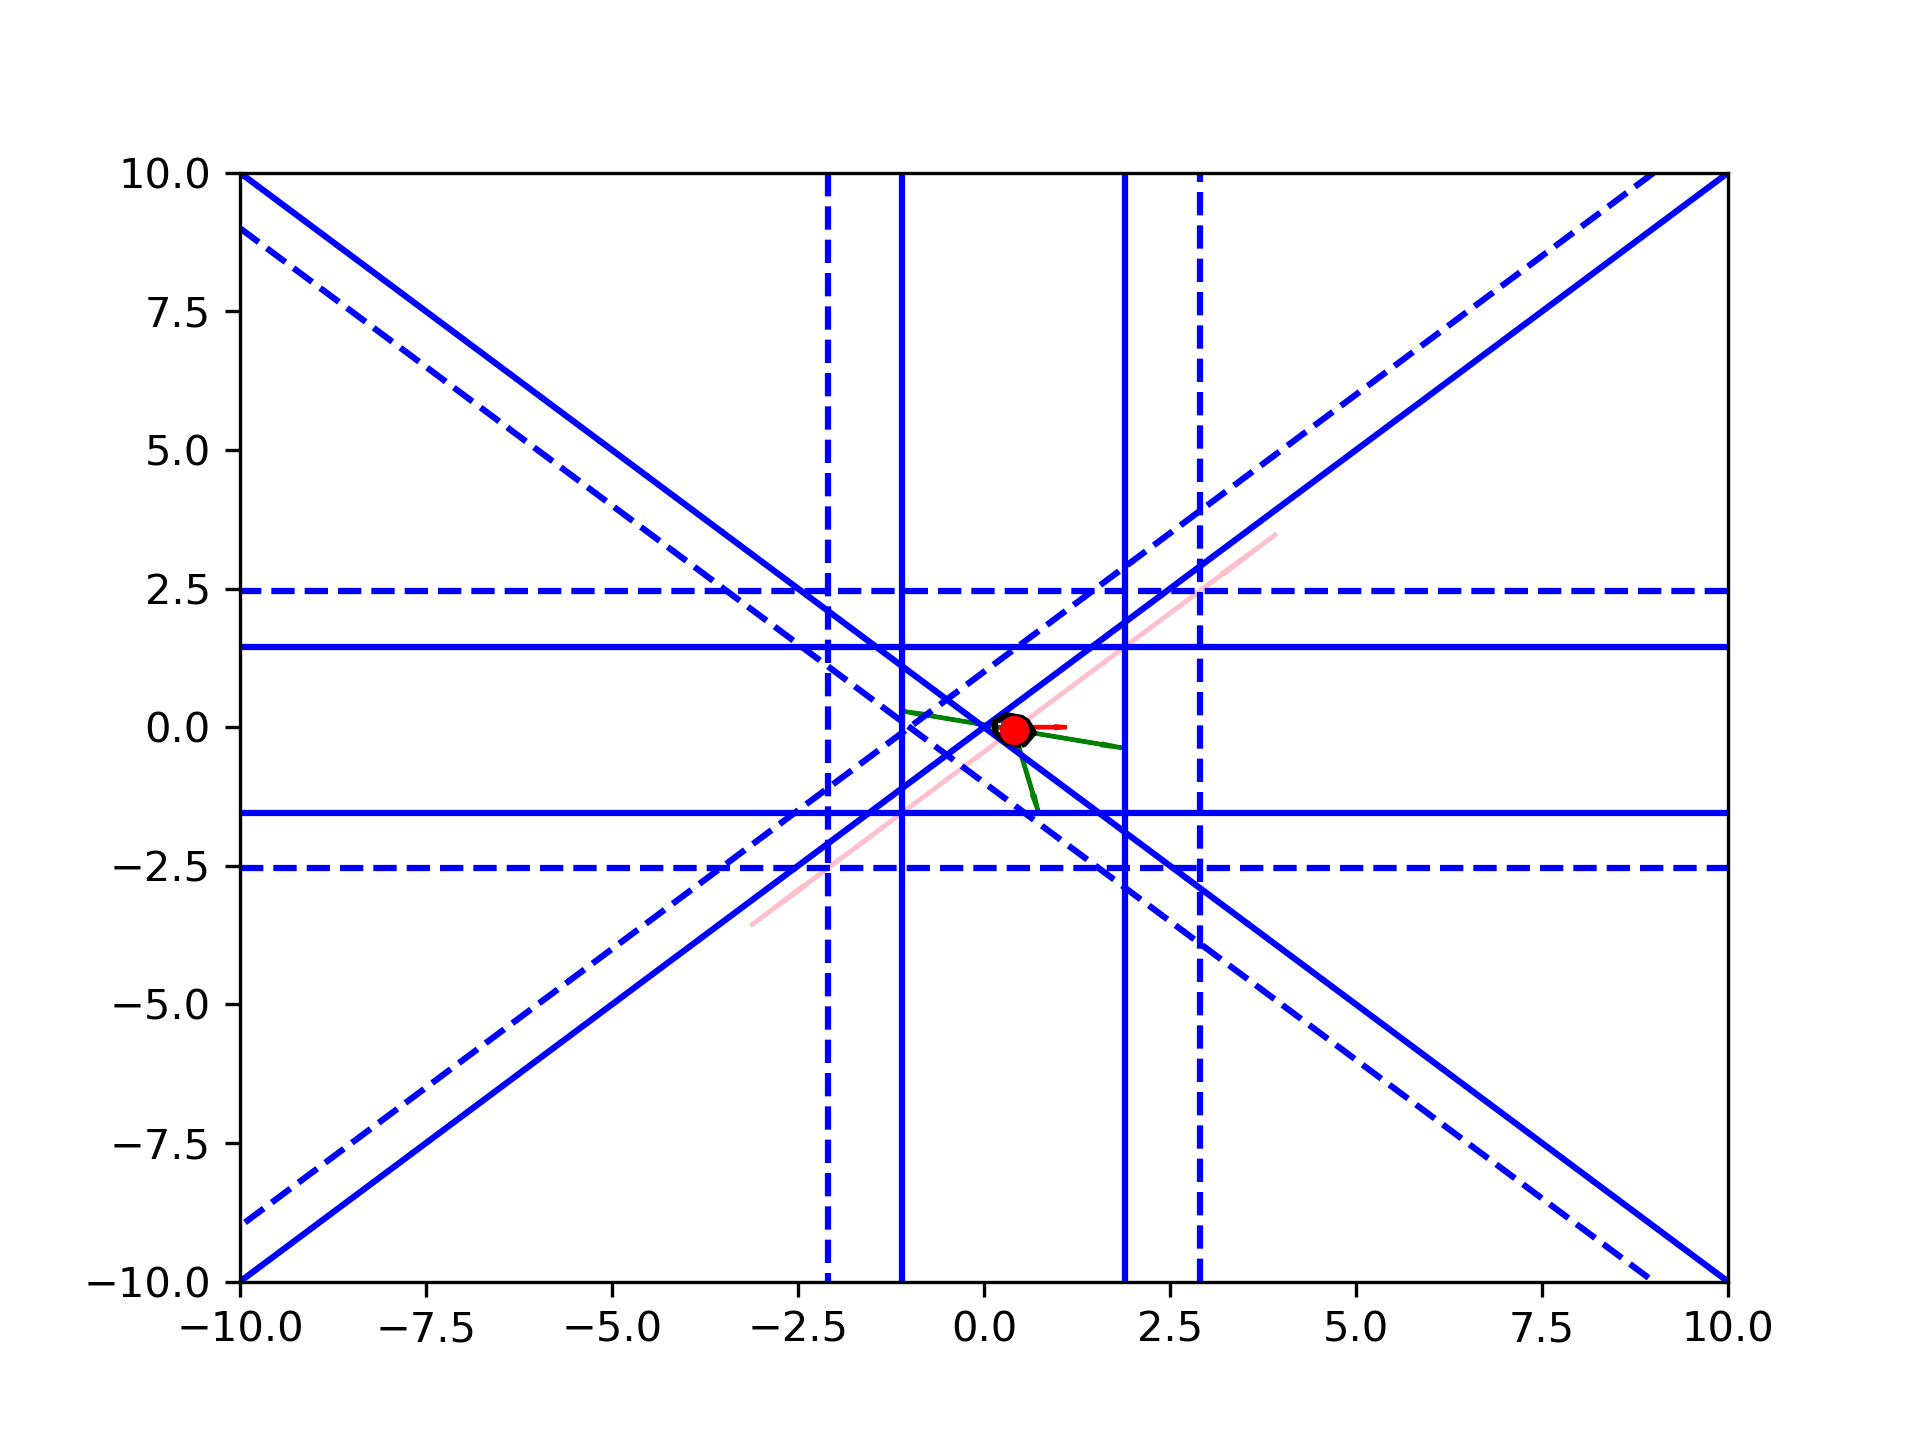
\includegraphics[scale=0.4]{images/everything_runs_1.png}
    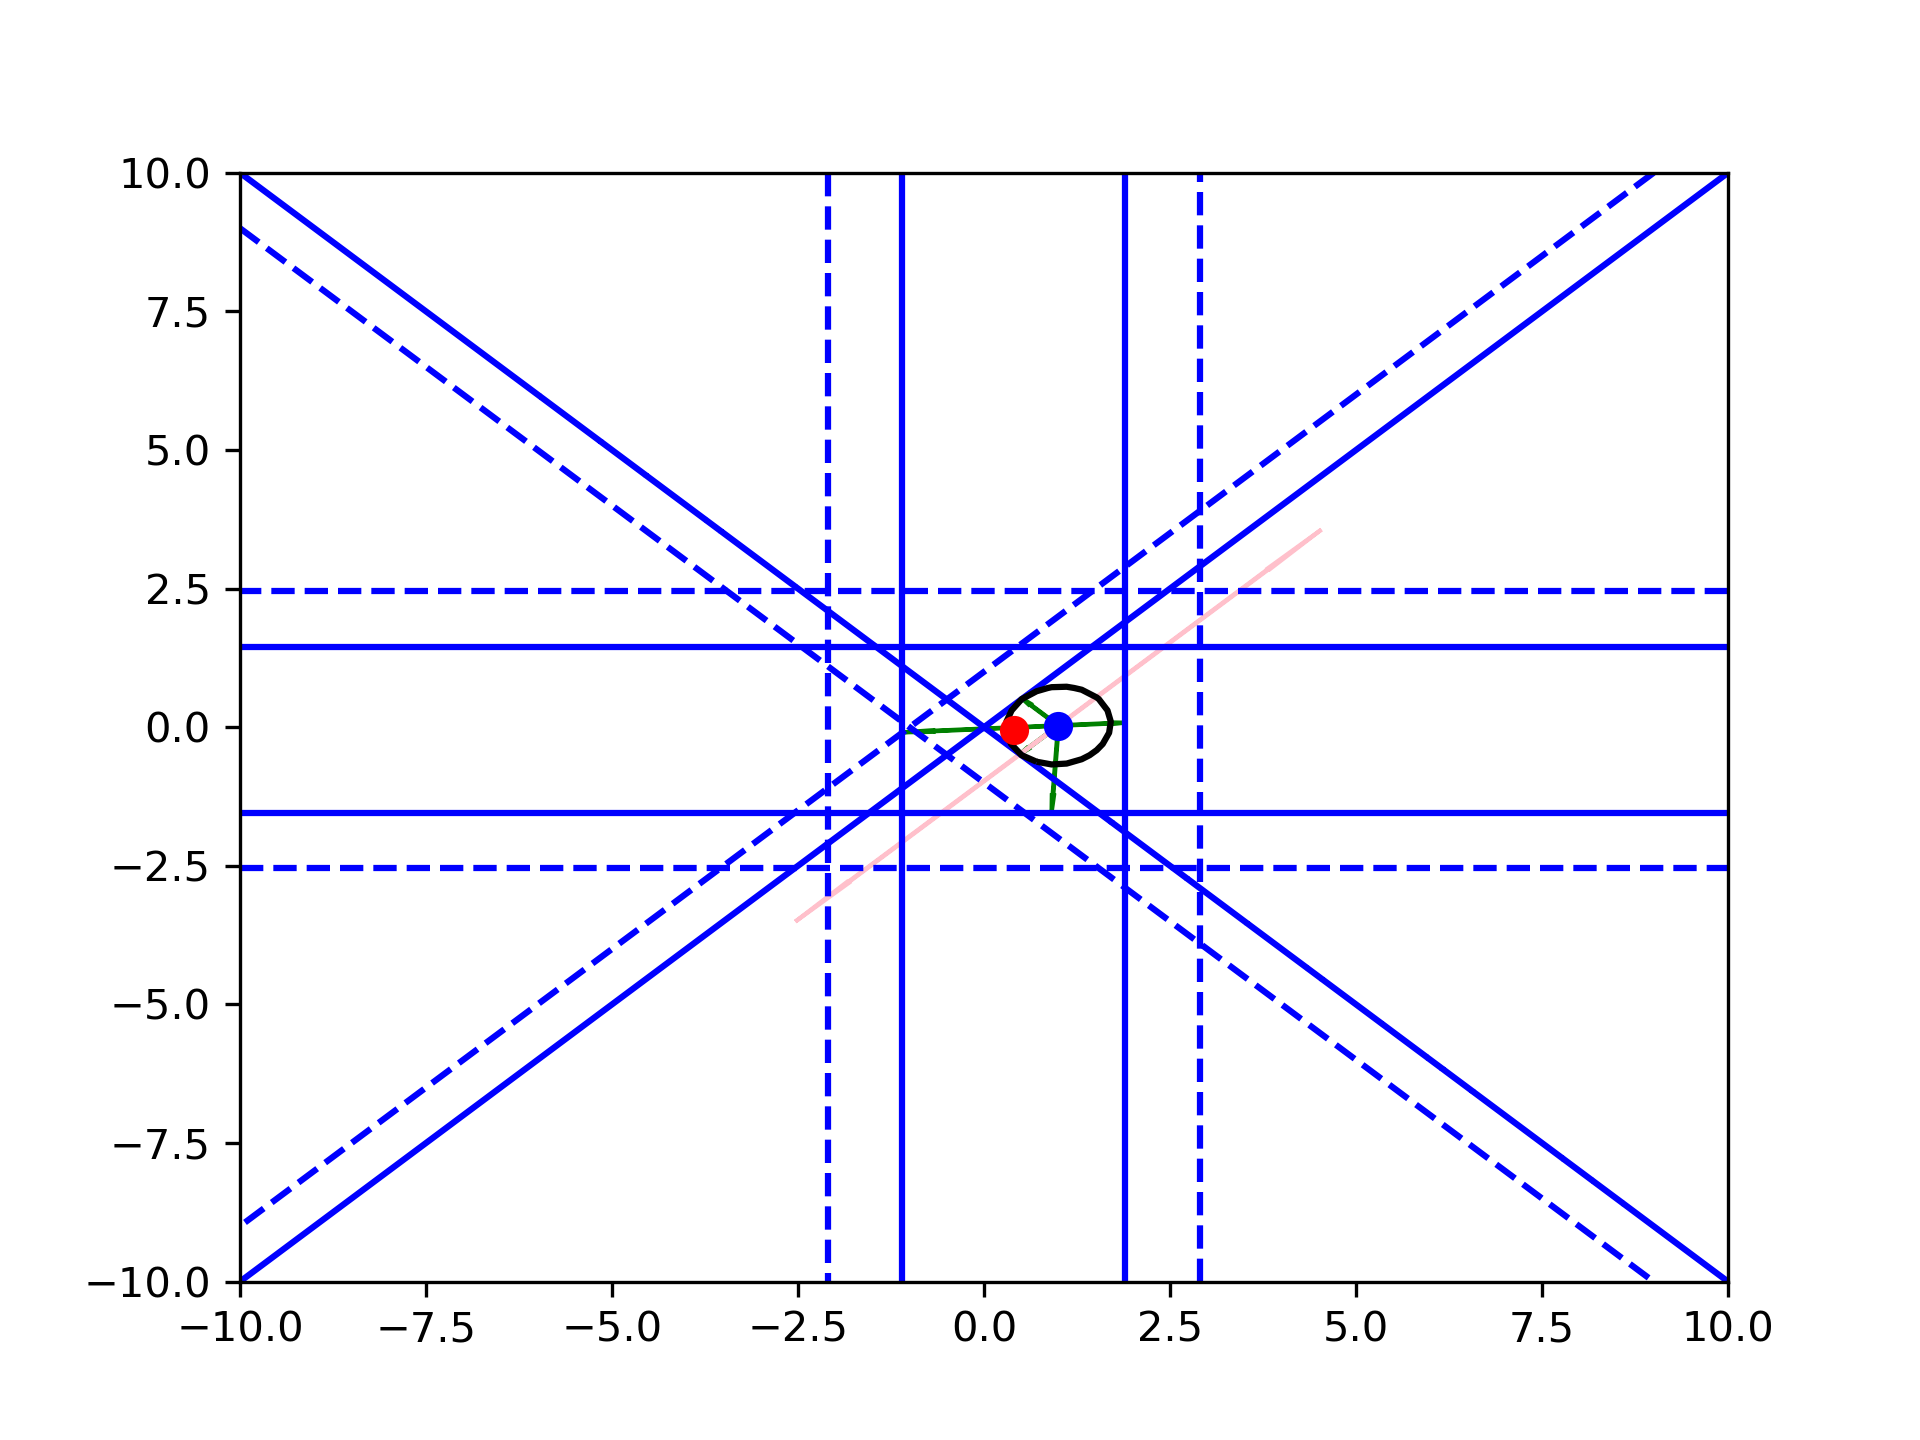
\includegraphics[scale=0.4]{images/everything_runs_2.png}
    \caption[An example of how the search for the sample region center can go wrong.]{An example of how the search for the feasible region center can go wrong.  
     On the left, a very small sample region is selected; however its proximity to the the minimizer over the outer trust region makes the model more accurate at the minimizer.
    	On the right, a sample region with larger volume is chosen, but it is further from the trust region minimizer.
	}
    \label{ellipse_runs_away}
\end{figure}


\subsubsection{Path Searches}

\sbnote{This discussion is quite vague, and in my opinion, off target.   You don't necessarily want to be moving toward a vertex.   You just don't want your ellipsoid to move in the opposite direction as   the descent direction.}

Although $\mfk$'s minimizer over $\outertrk$  can appear anywhere, there are some reasons for expecting it to be at a ``vertex."
If it lies in the interior, there is little need for using constrained approaches once near the solution.


%The ellipsoid with maximum volume, however, tends to lead $ \sampletrk $ away from vertices.
One way of trying to ensure a feasible direction towards a vertex, while still allowing a larger volume ellipsoid, is by limiting the search for the new center to lie on piecewise linear path starting at the current iterate $\xk$.

For example, our first attempt was to simply search a line directed orthogonally away from the closest constraint.
This has obvious problems as shown in \cref{first_line_search}: we should avoid letting the new center get closer to another constraint.    \sbnote{This could be clearer.   A key point is that with this method, you can determine the ellipsoid center simply by moving along this line until you are equi-distant from the 2 closest constraints.  Thus,  there is little gain if the current iterate is close to two or more constraints.}

\begin{figure}[ht]
    \centering
    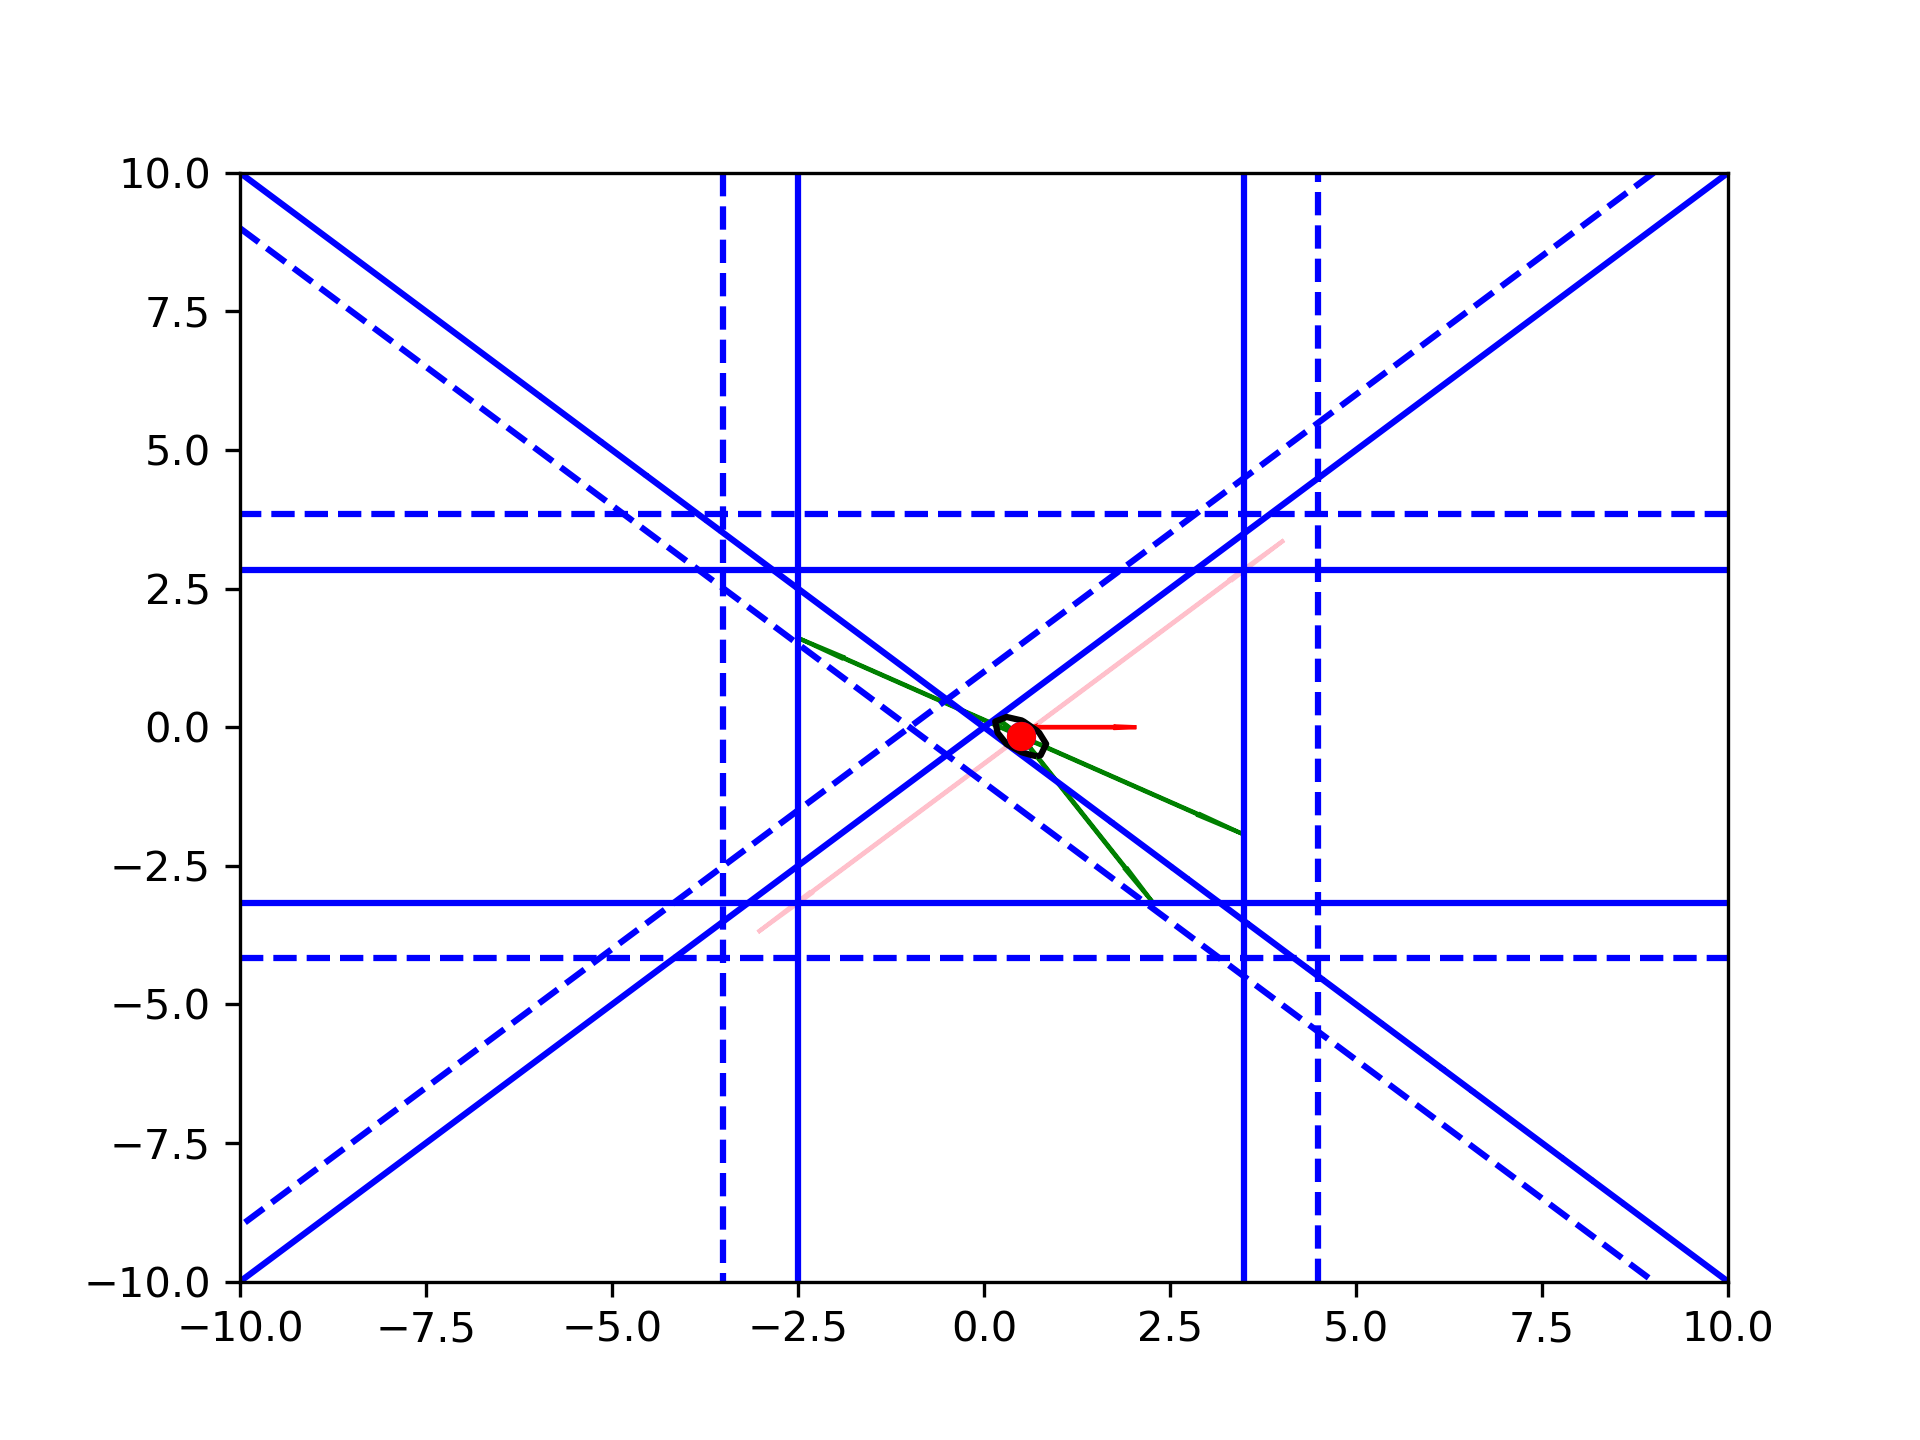
\includegraphics[scale=0.4]{images/line_1.png}
    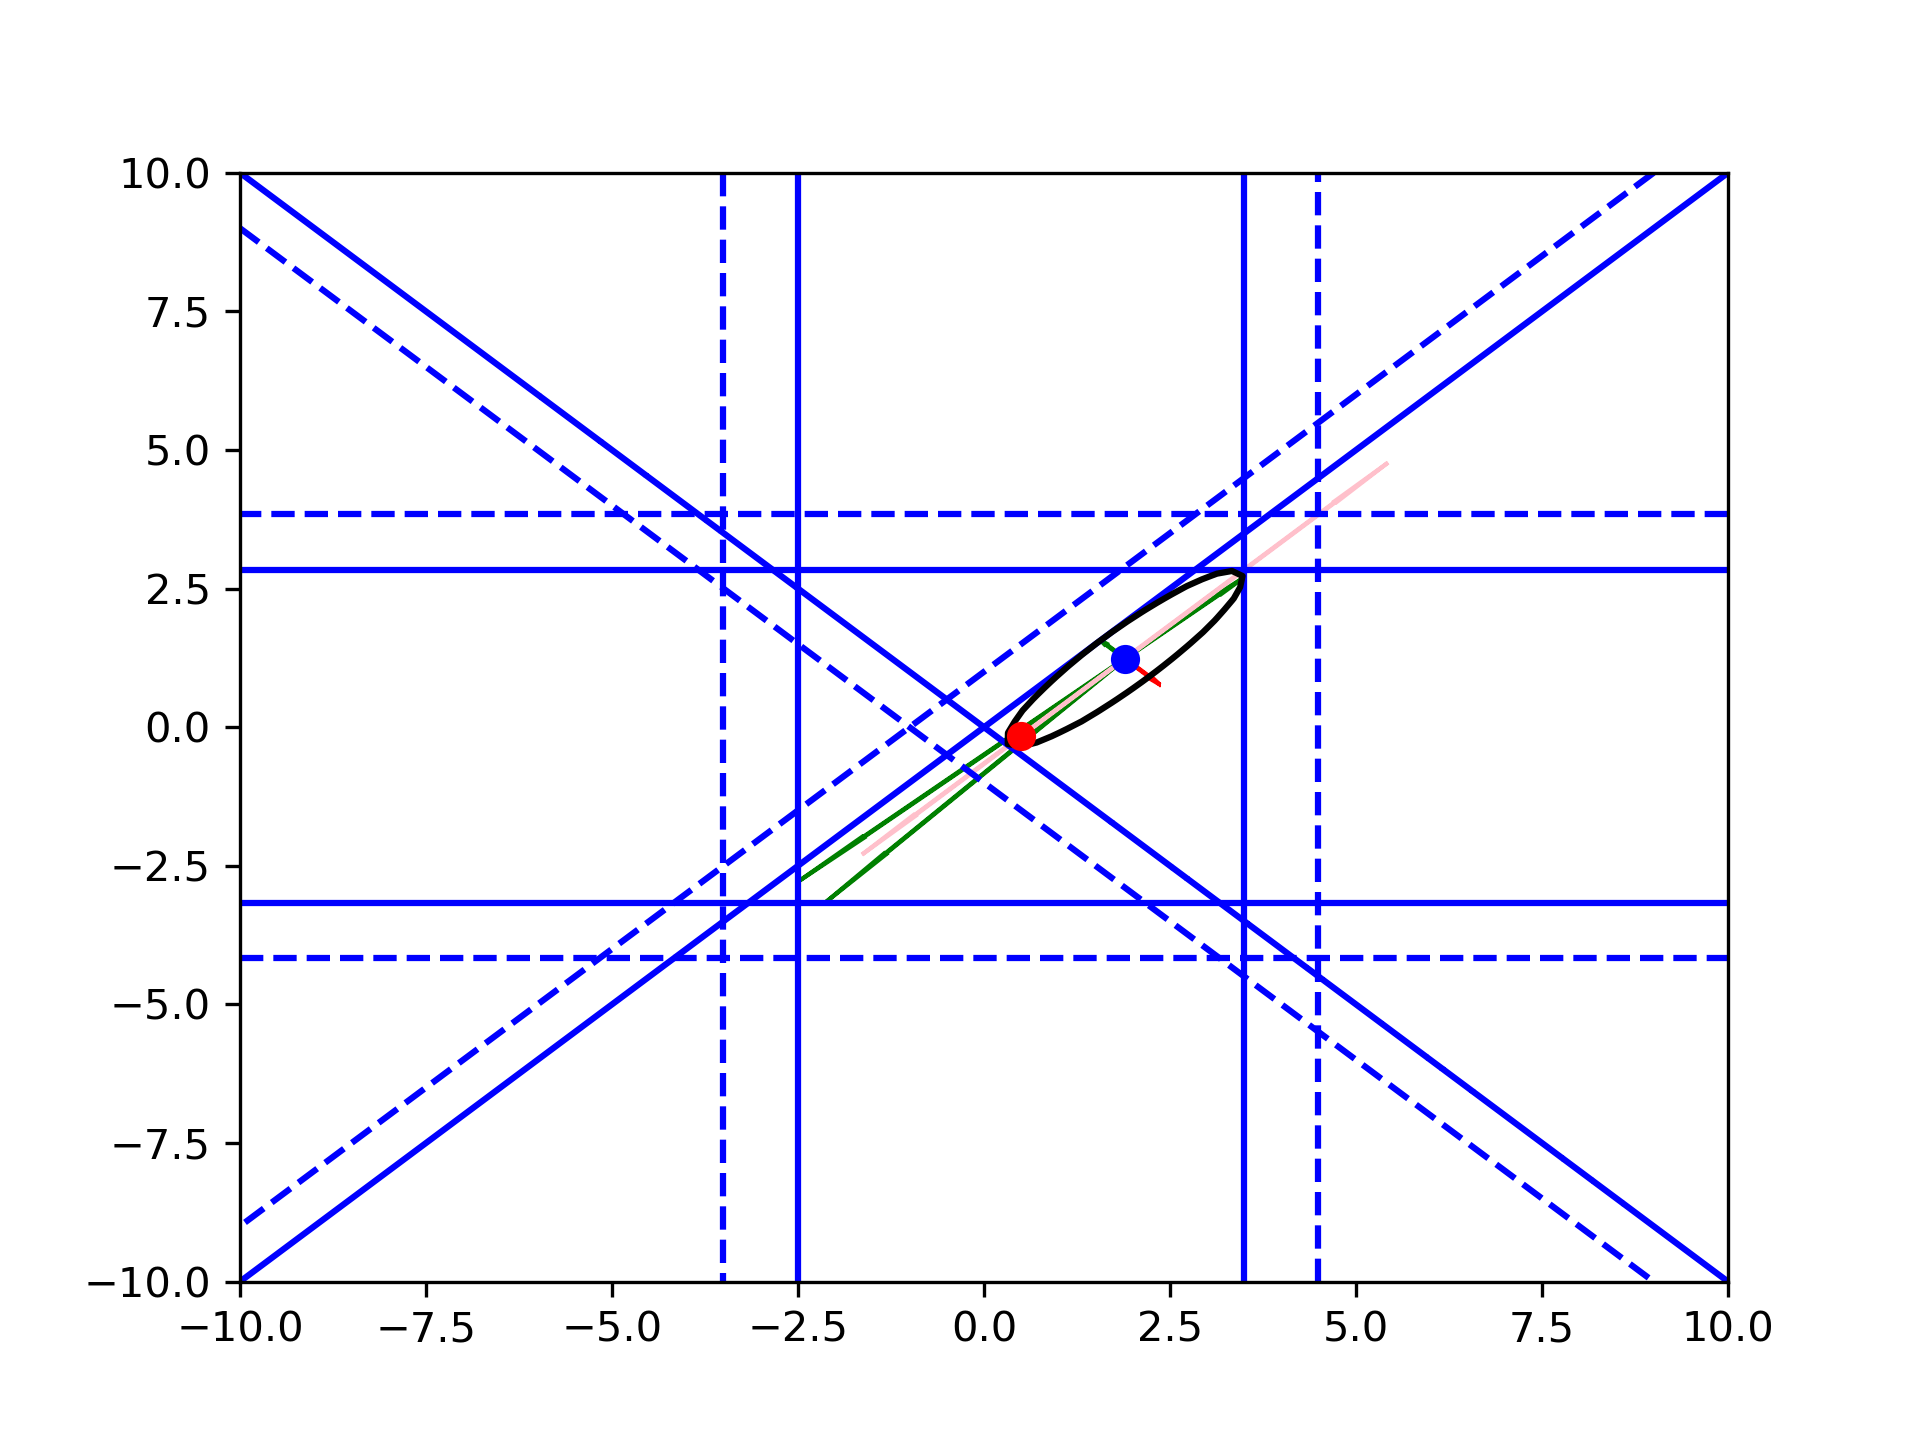
\includegraphics[scale=0.4]{images/line_2.png}
    \caption[Why only considering the nearest constraint is not sufficient. ]
        {Why only considering the nearest constraint is not sufficient.   On the left is the starting ellipsoid.
    	By choosing centers further away from only the nearest constraint, the ellipsoid becomes narrow as another constraint is limiting the length of the second axis.
	}
    \label{first_line_search}
\end{figure}

To fix this, we search along a piecewise linear path leading away from the closest constraints.   
The algorithm works by choosing a set of points $s_1, s_2, \ldots, s_{n_{\text{points}}}$ that are each equidistant to a subset of the constraint's faces.
The center search then considers points along the line segments between these points.
% Namely, it starts at the current iterate and travels along a ray away from all the closest constraints until it reaches a point equidistant to yet another constraint.

More precisely, the first point is chosen to be the current iterate: $s_1 = \xk$.
The algorithm then repeats the following process for $i$ from $1$ to $n_{\text{points}}$.  \sbnote{The following description is a little hard to follow.  Can we turn this into an algorithm?}
First, compute the set of nearest constraints, where the distance from a point $x$ to a constraint $A_i$ is given by $d(A_i, x) = \frac {|A_i x - b|}{\|A_i\|}$.
While finding the next point $s_{i+1}$, let  $A_E$ be a normalized array of the equidistant faces \sbnote{these are not faces.  These are normal vectors to the faces.}   $\{\frac{A_i}{\|A_i\|} | d(A_i, s_i) = \min_j d(A_j, s_i), i = 1, 2, \ldots, m\}$ and $b_E$ be the rows' corresponding values of $b$.
All other faces are called the remaining faces, and construct the matrix $A_R$ and vector $b_R$.
It \sbnote{what is ``it''?} then finds a search direction $p  = r{A_E}^T$ as a linear combination of the normal vectors to the equidistant faces.
%When the constraint violation of $s_i$ is non-zero, this search ray can be found by finding the point that doubles the current slack ${A_E}s_i-{b_E}$.
%This is given by $r{A_E}^T$ where $r$ solves the linear system ${A_E}(s_i + r{A_E}^T) - b_E = 2 ({A_E}n_i - b_E)$.
%If the current violation is zero, then the right hand side can be set to a vector of all ones to ensure that all slacks violations are the same: $A_E(s_i + r{A_E}^T) - b_E = 1$.
This search ray can be found by setting the slack to each equidistant face to a vector of all ones: $A_E(s_i + r{A_E}^T) - b_E = 1$.
We can travel along this ray until we reach a point that is the same distance to a remaining face.
Specifically, we can travel by 
\begin{align}
t = \argmin_j {\frac{d({A_E}_0, s_i) - d({A_R}_j, s_i)}{ {A_R}_j - d({A_E}_0) p} | ({A_R}_j - d({A_E}_0) p > 0 }. 
\end{align}

We can then set $s_{i+1} = s_{i} + t p$.

Of course, $n_{\text{points}}$ must be less than or equal to $n + 1$ in order for this to be defined.
Also, the algorithm must stop early if $A_E$ contains parallel faces.  \sbnote{say more about this.  why must it stop early?}

% if we let $\nabla \modelconstrainti\left(\xk\right) = A_i$ be the $i$th row of $A$, then we define the distance from a search point $s$ so the $i$th constraint to be


This means that we can define a class of searches that each limit the number of line segments to search $n_{\text{points}}$.  \sbnote{are you actually searching the line segments, or just the breakpoints $s_1, \ldots,s_{n_{\text{points}}}$?}

In \cref{line_can_run}, the red line shows the line segments equidistant from their closest constraints.
Notice that with two line segments, the algorithm can already choose new centers further from the vertex.

% TODO: REPLACE PICTURES
\begin{figure}[ht]
    \centering
    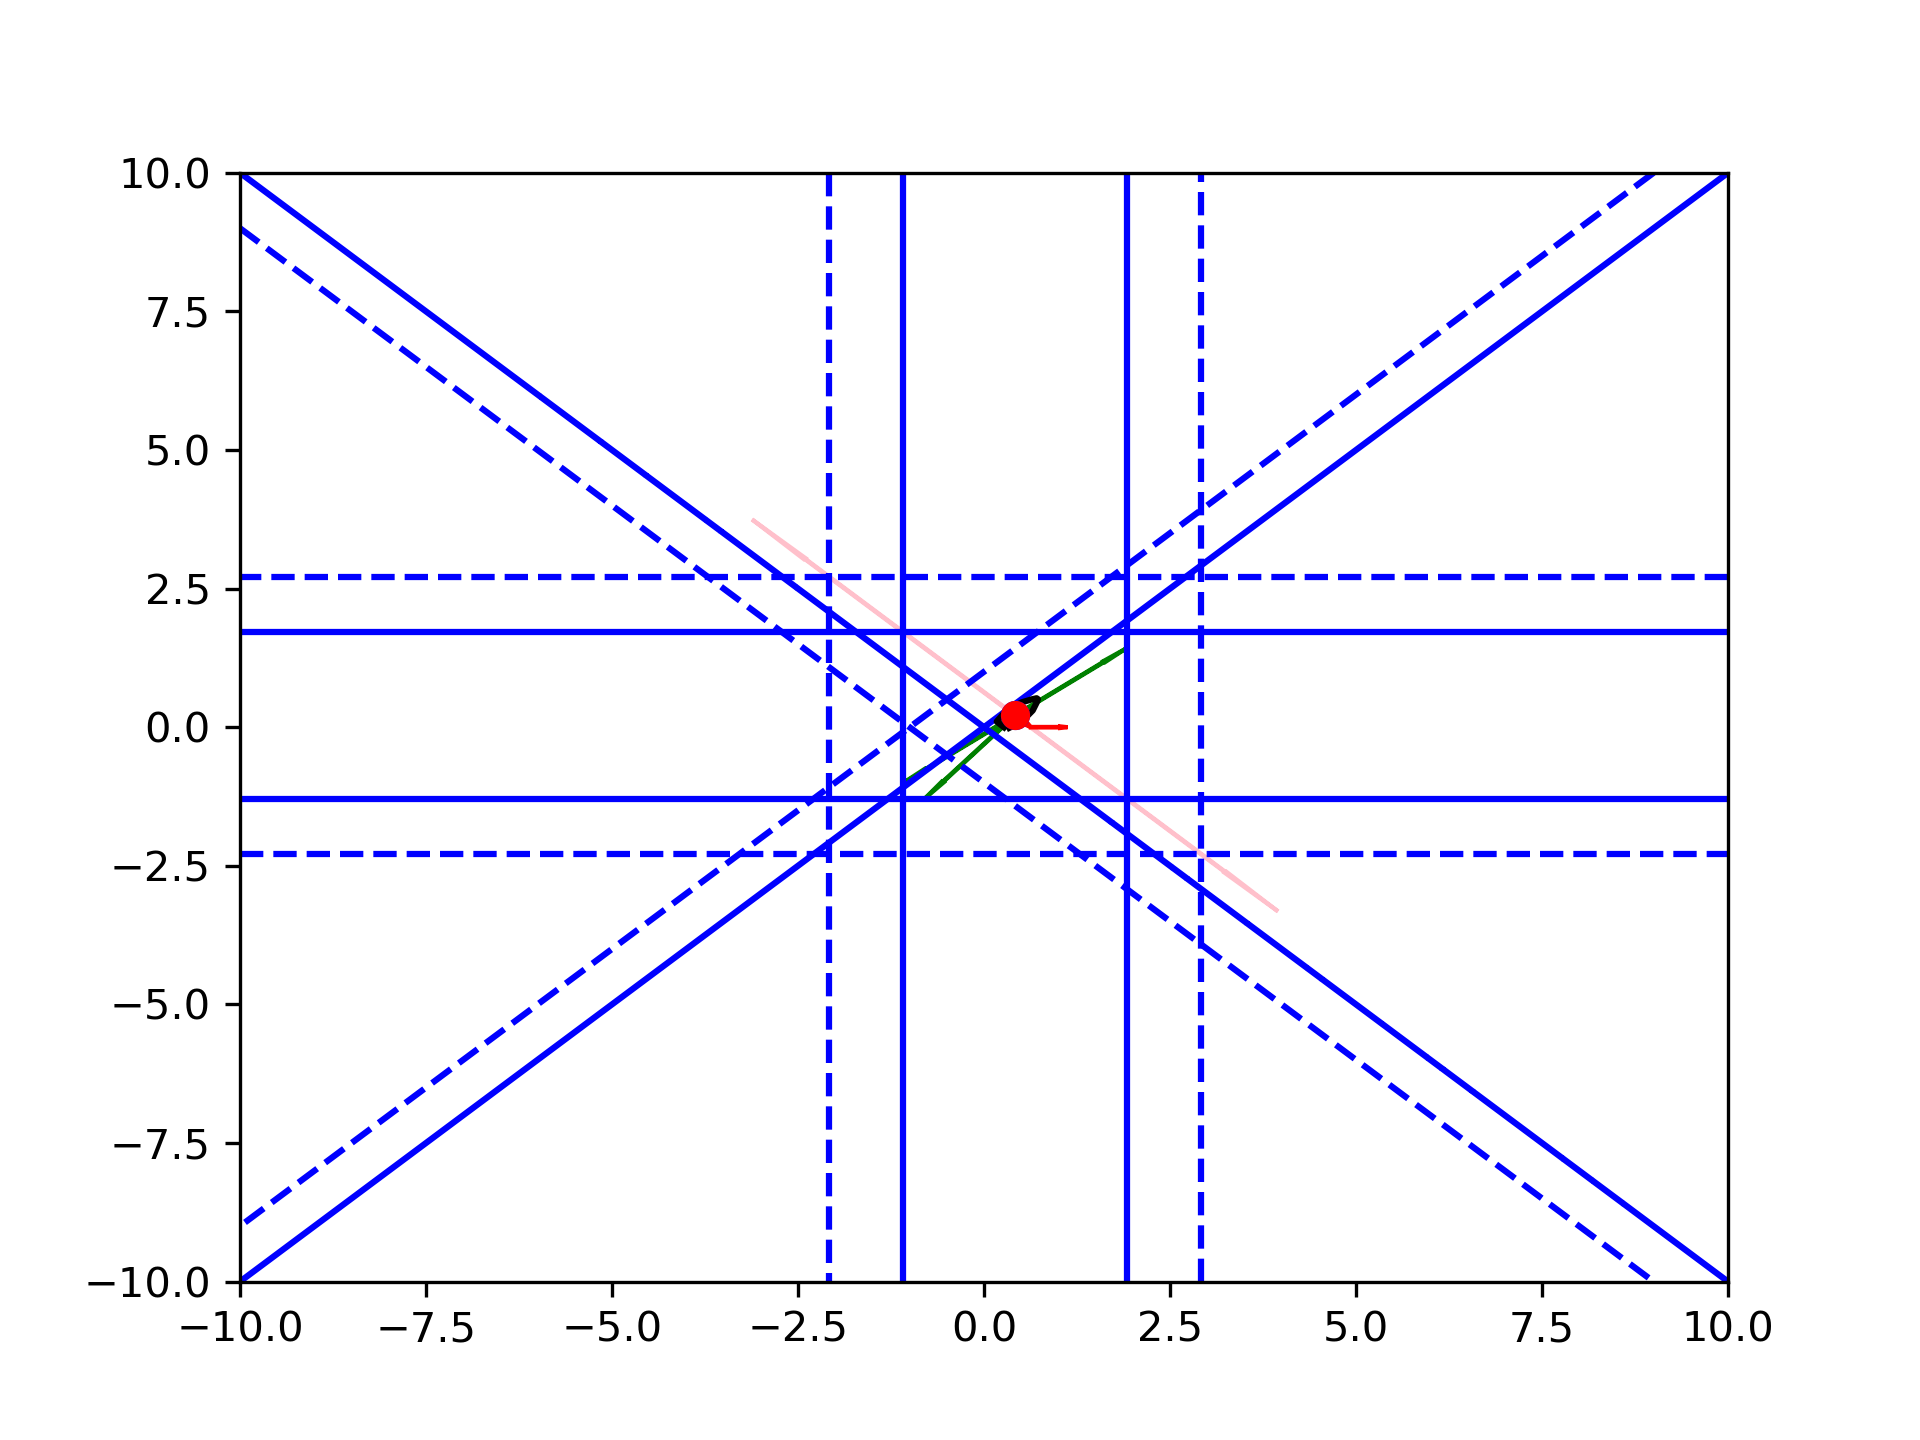
\includegraphics[scale=0.4]{images/run_away_1.png}
    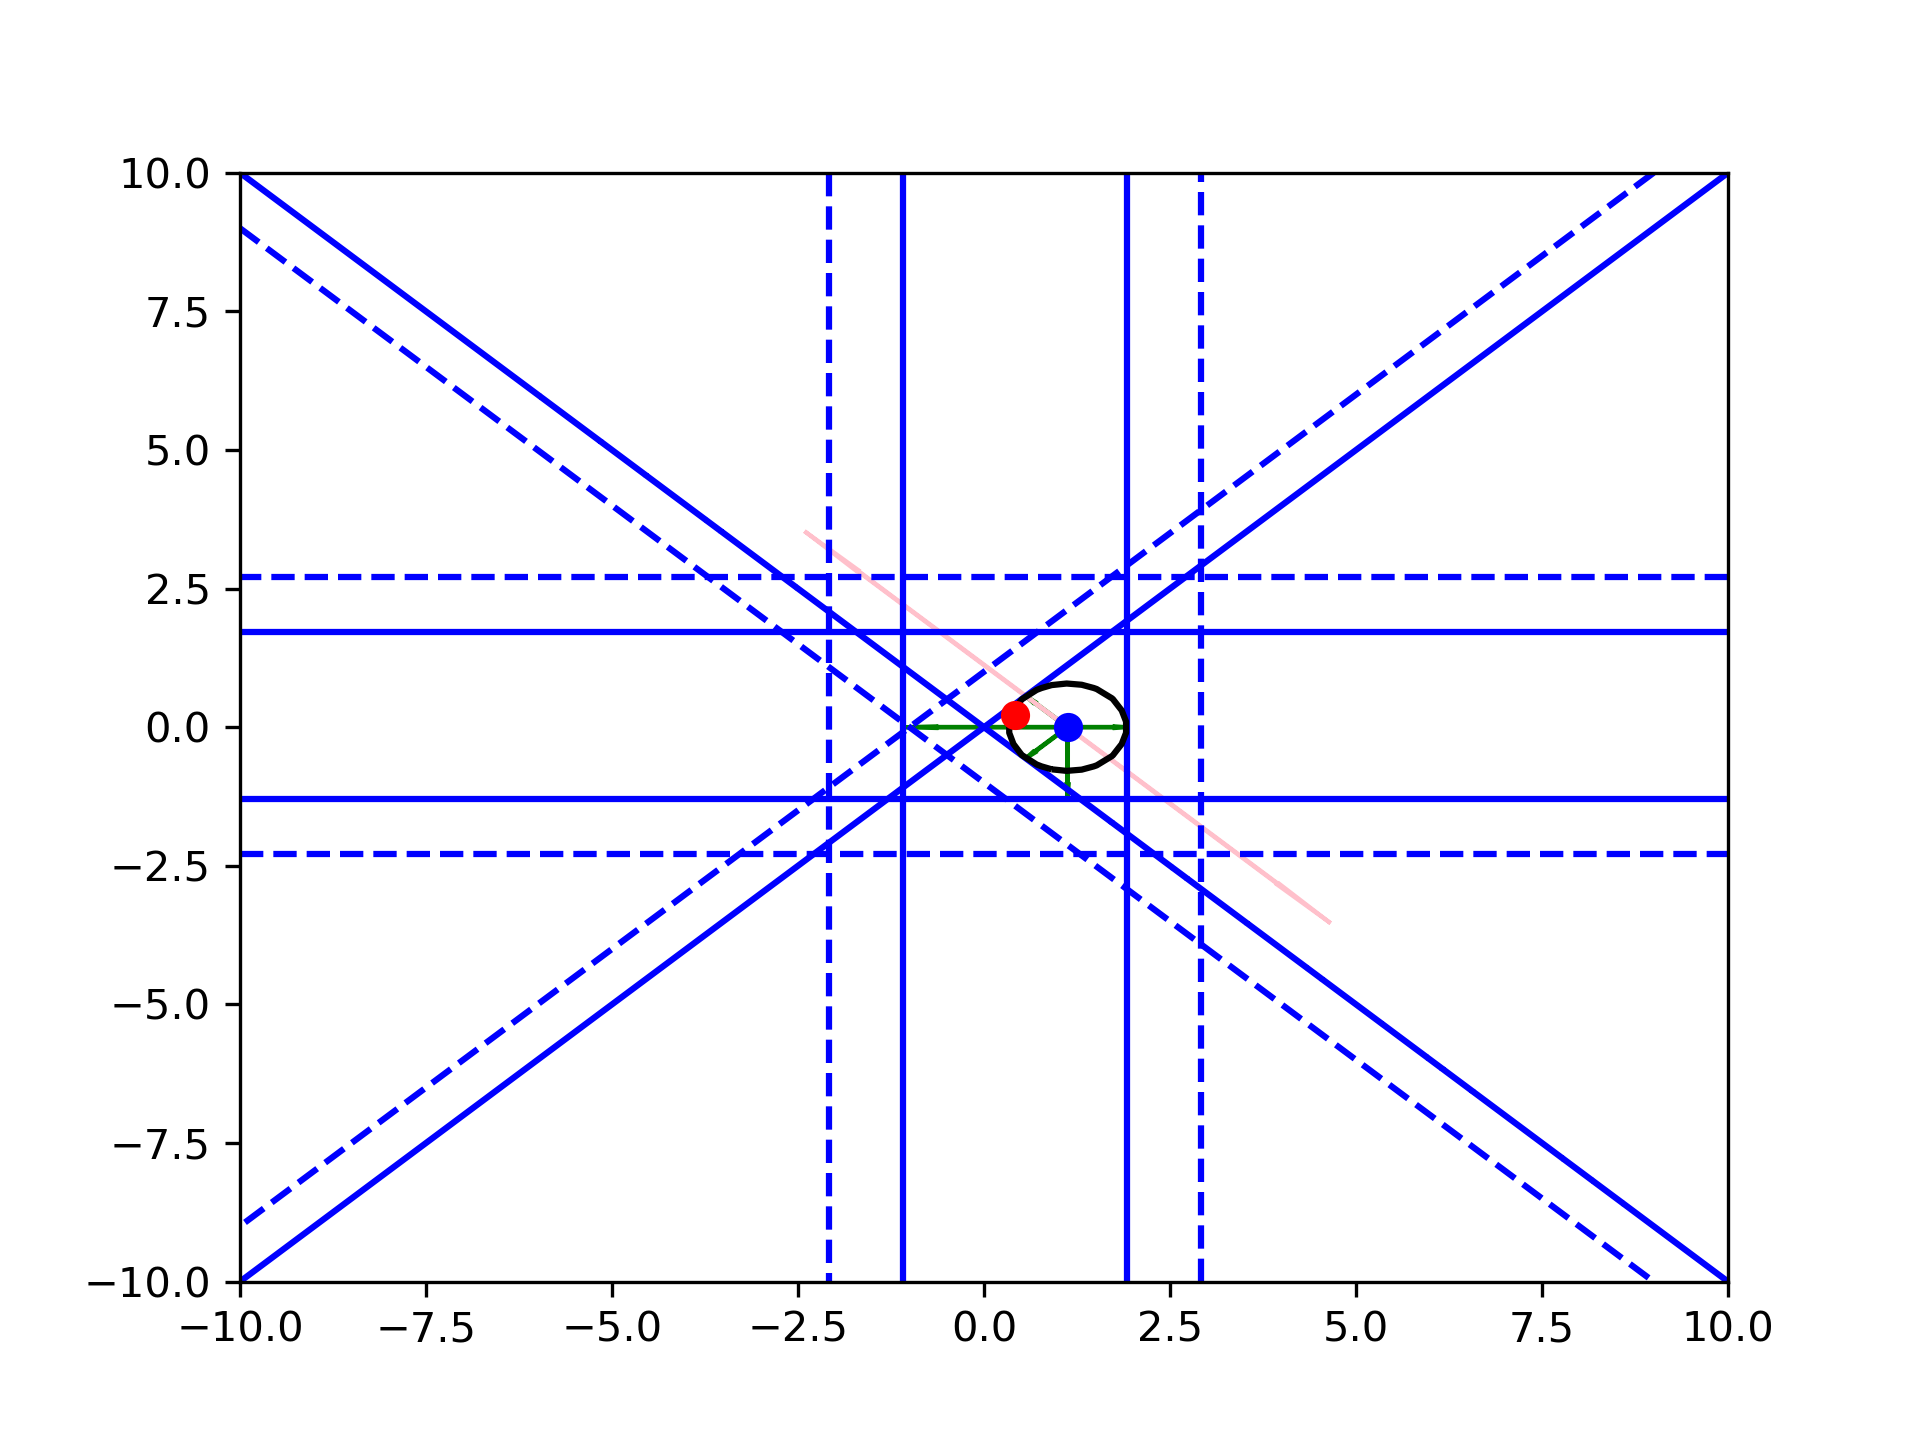
\includegraphics[scale=0.4]{images/run_away_2.png}
    \caption{
%     	\emph{Short:} Why only considering the nearest constraint is not sufficient. 
%     	\emph{Long:} On the left is the starting ellipsoid.
%     	By choosing centers further away from only the nearest constraint, the ellipsoid becomes narrow as another constraint is limiting the length of the second axis.
    Ellipse runs away from the optimizer}
    \label{line_can_run}
\end{figure}


\subsubsection{Ensuring the current iterate is in the trust region}
One potential difficulty created by moving the ellipsoid center is that the current iterate may not lie within the resulting ellipsoid.   
 \sbnote{This raises a number of questions.   First is whether the current iterate will be a sample point.    If it isn't, then the model function may disagree with the true function at the current iterate, so descent of the model function may not correspond to descent of the true function, even for very small steps.   Also, if the search region is chosen to be equal to the ellipsoidal region, then we may not be able to get descent at all.   At the end of the day,  we don't necessarily need the current iterate to be in the ellipsoid as long as 1) it is within the search trust region, and 2) the model function is sufficiently accurate over the search trust region.  Actually, we don't even need 2), do we?  We just need the accuracy condition to be satisfied at the current iterate, right?}



If $\xk \not \in \searchtrk $, the ellipse may not even contain a point with any reduction.
Thus, we have implemented a few ways of ensuring the current iterate is within the search trust region.
This can be done by either of the following two options:
\begin{itemize}
\item Adding a constraint to the ellipsoid problem to include the original point.
\item Expand the size of the ellipsoid.
\end{itemize}

%IMAGES GO HERE

\paragraph*{Adding a constraint.}
In order to include the original point as a constraint, we add a constraint of the following form to the definition of the ellipsoid.
\begin{align*}
\frac 1 2 \left(\xk - \ck\right)^T\qk\left(\xk - \ck\right) \le \frac 1 2 \sdk^2.
\end{align*}
Constraints of this nature make finding the ellipsoid much more expensive:
the optimization problem we construct uses ${\qk}^{-1}$ as decision variables, so that constraints in terms of $\qk$ must model matrix inversion.

\paragraph*{Increase the size.}
An alternative is to scale $\qk$ by a constant.
We use the scaling factor $\sdk$ defined by
\begin{align*}
\sdk = \max \left\{1, \sqrt{\left(\xk - \ck \right)^T \qk \left(\xk - \ck \right)} \right\}
\end{align*}
and let the ellipsoid be:
\begin{align*}
\ellipsek = \left\{x \in \Rn \bigg| \frac 1 2 \left(x - \ck\right)^T \qk \left(x - \ck\right) \le \frac 1 2 \sdk^2\right\}
\end{align*}
However, this means that in general $\ellipsek \not \subset \feasible$ so that the trust region subproblem must contain constraints for both the ellipsoid and the feasible region: 
$\searchtrk = \ellipsek \cap \feasiblek$.



\subsection{Convergence Analysis}
\label{linear_convergence_discussion}
Here,  we analyze the convergence behavior for one version of \cref{linearly_constrained_dfo}; namely the ellipsoidal method with a particular choice of the sample trust region $\sampletrk$  discussed below, and with $\searchtrk = \outertrk \cap \feasible$.    For our analysis, we make the following assumptions about the problem and the model functions:

\begin{assumption}
\label{for_fully_quadratic}
\label{lipschitz_hessian}
The function $f$ is twice continuously differentiable with Lipschitz continuous Hessian in $\domain$.   That is, there exists constant $\liphess > 0$ such that 
\begin{align}
\left\|\nabla^2 f(x) - \nabla^2 f(y)\right\| \le \liphess \left\|x - y\right\| \quad \forall x, y \in \domain.
\end{align}
\end{assumption}



\begin{assumption}
\label{lower_bound}
The function $f$ is bounded below over $\domain$.
That is,
\begin{align}
f(x) \ge \fmin \quad \forall x \in \domain.
\end{align}
\end{assumption}

\begin{assumption}
\label{interior_point}
There exists a point $\bar x$ within the interior of the feasible region.
Namely, using $\lca$ and $\lcb$ from \cref{the_constraints_are_linear}:
\begin{align}
\lca \bar x < \lcb.
\end{align}
\end{assumption}


\begin{assumption}
\label{uniformly_bounded_hessians_of_mf}
The Hessian's of $\mfk$ are uniformly bounded.  That is, there exists a constant $\beta \ge 1$ such that   \sbnote{Can we get rid of this assumption?}
\begin{align}
\left\|\nabla^2 \mfk\left(\xk\right)\right\| \le \beta - 1\quad \forall k \ge 0.
\end{align}
\end{assumption}






%
%With this modest assumption, we can make the assumptions more straightforward by replacing \cref{uniformly_bounded_hessians_of_mf} with \cref{uniformly_bounded_hessians_of_f}:





% \begin{assumption}
% \label{accuracy_assumption}
% There exists a constant $\delta_g$ such that 
% \begin{align}
% \|\nabla m_k\left(\xk\right) - \nabla f\left(\xk\right)\| \le \delta_g \dk \;\forall k \ge 0.
% \end{align}
% \end{assumption}




\sbnote{I think we can delete the following two assumptions}
\begin{assumption}  \sbnote{This does not need to be stated as an assumption, since this is the definition of our problem (in the linear case)}.
\label{the_constraints_are_linear}
The feasible region is described by linear constraints.
That is, we assume that there is an $m \times n$ matrix $\lca$ and vector $\lcb \in \Rm$ such that:
\begin{align*}
\feasible = \left\{x \in \Rn \bigg | \lca x \le \lcb \right\}
\end{align*}
\end{assumption}

\begin{assumption}  \sbnote{We don't need this assumption, since this is a consequence of bounded Hessians of $f$}.
\label{lipschitz_gradient}
The function $f$ is differentiable and its gradient $\nabla f$ is Lipschitz continuous with constant $\lipgrad > 0$ in $\domain$.
That is,
\begin{align}
\|\nabla f(x) - \nabla f(y)\| \le \lipgrad \|x - y\| \quad \forall x, y \in \domain.
\end{align}
\end{assumption}


Our analysis follows closely that of  \cite{doi:10.1080/10556788.2015.1026968}, which presents a class of trust region algorithms for derivative-free optimization with convex constraints.      \sbnote{Check this reference.   I think you might mean the other paper by Conejo et. al}.   Indeed, if 
the tolerances $\tau_{\chi}$ and $\tau_{\Delta}$ are set to zero,  then \cref{linearly_constrained_dfo} is a particular implementation of the algorithm studied in \cite{doi:10.1080/10556788.2015.1026968}.  It is therefore sufficient to show that the model functions generated by our method satisfy the hypotheses required in \cite{doi:10.1080/10556788.2015.1026968}.  

Specifically, the following hypotheses must be satisfied:
\begin{itemize}
\item[$H_0$] There exists a constant $\kappa_f$ such that the following efficiency condition is satisfied for all $k$:
\begin{align}
\label{efficiency}
\mfk\left(\xk\right) - \mfk\left(\xk + \sk\right) \ge \kappa_f \chi_k \min\left\{ \frac{\chi_k}{1+\|\nabla^2 \mfk(\xk)\|}, \dk, 1 \right\},
\end{align}
where $\chi_k$ is the criticality measure defined by \cref{?}.  \sbnote{I don't think you have given a precise definition of $\chi_k$ anywhere for the linear problem}.
\item[$H_1$] The function $f$ is differentiable and its gradient $\nabla f$ is Lipchitz continuous with constant $L > 0$ in $\domain$.
\item[$H_2$] The function $f$ is bounded below over $\domain$.
\item[$H_3$] The matrices $H_k$ are uniformly bounded. That is, there exists a constant $\beta \ge 1$ such that $\|\nabla^2 \mfk(x)\| \le \beta - 1$ for all $k \ge 0$ \sbnote{and $x \in \Omega$?}
 \sbnote{Is it assumed that $\mfk$ is a quadratic function with Hessian $H_k$?}
\item[$H_4$] There exists a constant $\delta_g$ such that $\left\|\nabla m_k\left(\xk\right) - \nabla f\left(\xk\right)\right\| \le \delta_g \dk$ for all $k \ge 0$.
\end{itemize}

Observe that $H_1$ and $H_2$ are equivalent to Assumptions \ref{lipschitz_hessian} and \ref{lower_bound}, respectively.   For $H_0$,  \cite{Conn:2000:TM:357813} showed that the Generalized Cauchy Point satisfies \cref{efficiency}.  Thus, the solution of the trust region subproblem must also satisfy \cref{efficiency}.

\sbnote{Let's be careful here.   Is $\chi_k$ the criticality measure for the model function, or the criticality measure for the original problem?}  \sbnote{Also, note that in the statement of our algorithm, $s^{(k)}$ is the minimizer of the model function over $\searchtrk$ rather than the Cauchy point. }  

The following lemma shows that $H_3$ is satisfied under our assumptions:

%
%Here, we let $\domain$ be some open set containing the feasible region: $\feasible \subset \domain$.  \sbnote{Do we really need $\domain$?}





%
\subsection{Satisfying the assumptions}

\subsubsection{Simplified Third Hypothesis}
\label{simpler_h3}
First, we show that \cref{uniformly_bounded_hessians_of_f} can be used instead of \cref{uniformly_bounded_hessians_of_mf} under some restrictions.
Namely, for this to be true, we also first assume:
%
%
%
%This is the result of the following lemma:

\begin{assumption}
\label{uniformly_bounded_hessians_of_f}
The Hessian's of $f$ are uniformly bounded at each iterate. That is, there exists a constant $\beta \ge 1$ such that
\begin{align*}
\left\|\nabla^2 f\left(\xk\right)\right\| \le \beta - 1\quad \forall k \in \naturals
\end{align*}
\end{assumption}

\begin{assumption}
\label{delta_max}
There exists a $\dmax > 0$ such that $\dk \le \dmax$ for all $k \ge 0$.
\end{assumption}

\sbnote{The following lemma makes the assumption that the quadratic model function satisfies an error bound on the Hessian.  But this is only true if the model function defined by \cref{quadratic_errors} is built with a $\Lambda$-poised sample set.  So this needs to be stated explicitly in the lemma.} 
\begin{lemma}
\label[lemma]{replacing_h3}
Suppose that \cref{lipschitz_hessian}, \cref{delta_max}, and \cref{uniformly_bounded_hessians_of_f} hold.
Let $\mfk$ be a quadratic model of $f$ over $B_{\infty}(\xk, \dk)$  as in \cref{quadratic_errors} for each $k \in \naturals$.
Then \cref{uniformly_bounded_hessians_of_mf} is also satisfied.
\end{lemma}

\begin{proof}
By \cref{uniformly_bounded_hessians_of_f}, we can choose $\beta_1 \ge 1$ to be such that for all $k \in\naturals$:
\begin{align*}
\left\|\nabla^2 f\left(\xk\right) \right\| \le \beta_1 - 1.
\end{align*}
% \cref{model_improving_algorithm},
Because $\mfk$ are fully quadratic by \cref{lipschitz_hessian}, we know that \cref{introduction_3_1} is satisfied.
Thus, we can apply \cref{quadratic_errors} to see that \cref{error_in_hessian} is satisfied.
Combining this with \cref{delta_max} we see that
\begin{align*}
\left\|\nabla^2 f\left(\xk\right) - \nabla^2 m_f\left(\xk\right) \right\| \le \kappa_{h} \dk \le \kappa_{h} \Delta_{\text{max}}
\end{align*}
Defining $\beta_2 = \kappa_{h} \Delta_{\text{max}} + \beta_1 \ge 1$, we see that
\begin{align*}
\left\|\nabla^2 m_{f}\left(\xk\right)\right\| \le \left\|\nabla^2 m_{f}\left(\xk\right) - \nabla^2 f\left(\xk\right)  \right\| + \left\|\nabla^2 f\left(\xk\right) \right\|
\le \beta_2 - 1 .
\end{align*}
\end{proof}

% For any $x \in \feasible$, we have that the set of gradients of active constraints is linearly independent. That is, the vectors $\{\nabla c_i(x) |  \forall i \in \activei(x)\}$ is linearly independent.


\subsubsection{Satisfying the Accuracy Assumption}
\label{satisfying_accuracy}
To show that the accuracy condition $H_4$ is satisfied, we need to impose some conditions on the ellipsoidal sample regions $\sampletrk$.     In particular, we require the ellipsoid to satisfy the following {\em suitability} condition:




%Because the ellipsoid we construct must be feasible with respect to both the trust region and the constraints,
%we simplify notation by creating a matrix $\lctra$ and vector $\lctrb$ from $\lca$ and $\lcb$ defined in \cref{the_constraints_are_linear} as follows:
%\begin{align}
%\polyk = \{x \in \Rn | \; \lca x \le \lcb, \|x - \xk\|_{\infty} \le \dk \} \label{polyhedron_k} 
%= \{x \in \Rn | \lctra x \le \lctrb, \|{\lctra}_i\| = 1 \}.
%\end{align}
%This is the normalized polyhedron formed by adding the trust region constraints for iteration $k$ to the problem constraints.
%
%As discussed in \cref{ellipsoidal_lambda}, we know that if the condition number of $\qk$ is bounded, 
%we can map a poised set over the unit ball to $\sampletrk$.
%However, we must also ensure that we are always able to find a feasible ellipsoid.
%Although it is not always possible to find a feasible ellipsoid that contains the current iterate,
%we can find a feasible ellipsoid that only needs to be scaled by a constant to do so.
%This ellipsoid must satisfy the following conditions:

\begin{definition}
\label{define_suitable_ellipsoid}
An ellipsoid $\ellipsek$ determined by a positive definite, symmetric matrix  $\qk$, a center $\ck \in \Rn$, and a radius $\sdk > 0$
is said to be a \textbf{suitable ellipsoid} for iteration $k$ if all of the following are satisfied:
\begin{itemize}
\item[1.] The ellipsoid $\ellipsek = \left\{x \in \Rn \bigg| \left(x - \ck\right)^T\qk\left(x - \ck\right) \le \frac 1 2 \sdk^2 \right\}$ 
satisfies $\ellipsek \subseteq \polyk$ as defined in \cref{polyhedron_k}
\item[2.] The ellipsoid $\scaledellipsek = \left\{x \in \Rn \bigg | \left(x - \ck\right)^T\qk\left(x - \ck\right) \le  \sdk^2 \right\}$ satisfies $\xk \in \scaledellipsek$.
\item[3.] $\condition \left(\qk\right)$ is bounded independently of $k$.

\sbnote{There is some inconsistency here.  If $\scaledellipsek$ is defined by radius $\delta_k$.  In contrast $\ellipsek$ is defined by radius $\delta_k/\sqrt{2}$.}
\end{itemize}
\end{definition}

\subsection{Finding a suitable ellipsoid}
This section shows how to construct an ellipsoid that satisfies \cref{define_suitable_ellipsoid}.  

\sbnote{Before proving anything, please give an algorithm for constructing the suitable ellipsoid.  My comments below may help.}


The active constraints at a point $x$ will be denoted by
\begin{align}
\activei(x) = \{1 \le i \le m | c_i(x) = 0 \Leftrightarrow {\lca}_ix = {\lcb}_i \} \label{define_activei}
\end{align}

We begin by defining a direction $\uk$ that is maximally feasible with respect to the active constraints.  To make this precise,   let $\lca$ be defined by \cref{the_constraints_are_linear} and $\mathcal S \subseteq \{1, \ldots, m\}$ be arbitrary.
Define:  \sbnote{The notation here is maddening.   $\alphaone$ is a direction,  whereas $\alphatwo$ and $\alphathree$ are scalars.    Maybe change $\alphaone$ to $u(\mathcal S)$ to make it more obvious that it is a direction. } 



\begin{align}
\alphaone (\mathcal S) = \begin{cases}
\argmax_{\|u\| = 1} \min_{i \in \mathcal S} -u^T{\lca}_i & \text{if} \; \mathcal S \ne \emptyset \\
\emptyset & \text{if} \; \mathcal S = \emptyset
\end{cases} \label{define_alpha_one} \\
\alphatwo(\mathcal S) = \begin{cases}
\max_{\|u\| = 1} \min_{i \in \mathcal S} -u^T{\lca}_i & \text{if} \; \mathcal S \ne \emptyset \\
1 & \text{if} \; \mathcal S = \emptyset
\end{cases} \label{define_alpha_two}\\
\alphathree(x) = \alphatwo\left(\activei(x)\right) \label{define_alpha_three} \\
\alpha_k =  \alphathree\left(\xk\right) \label{define_alpha_k} \\
\uk \in  \alphaone\left(\activei\left(\xk\right)\right) \label{define_u_k}
\end{align}
Here, $\alphathree$ is a set of directions that hopefully head away from each of the active constraints at a point.  \sbnote{No it isn't, it is a scalar!}

\sbnote{It looks to me that you don't need to be so general with the index set $\mathcal S$ above.    I think you only ever use $\mathcal S = \activei(\xk)$.   So maybe you could simplify notation by writing}
\[ \uk = \begin{cases}\argmax_{\|u\| = 1} \min_{i \in {\mathcal A}^{(k)}} -u^T{\lca}_i & \text{if} \; {\mathcal A}^{(k)} \ne \emptyset \\
0 & \text{if} \; {\mathcal A}^{(k)} = \emptyset
\end{cases}\]
and 
\[\displaystyle \alpha_k =
\begin{cases} =\min_{i \in {\mathcal A}^{(k)}} -(\uk)^T A_i & \text{if}\;  {\mathcal A}^{(k)} \ne \emptyset \\
1 & \text{if}  \; {\mathcal A}^{(k)} = \emptyset
\end{cases}\]
=================
To define a suitable ellipsoid, it will be convenient to define the rotation matrix
\begin{align}
\rotk = 2\frac{(e_1 + \uk)(e_1 +\uk)^T}{(e_1 +\uk)^T(e_1 +\uk)} - \boldsymbol I \label{define_r} \\
T_k(x) = \rotk\left(x - \xk\right) \label{define_affine_mapping}
\end{align}


\sbnote{Here is where you can describe the method for constructing the ellipsoid.  The following is a possible outline:}
\begin{itemize}
\item Let $L$ be the shortest distance from $\xk$ to any point on a non-active constraint.  
\item Define $\alpha'=\sqrt{(1+\alpha_k^2)(1+\frac{1}{\sqrt{2}})}$ and $\delta_f = \frac{1}{\alpha'}L$.  
\item Define the center of the ellipsoid as $c^{(k)} = \xk+\delta_f \uk$.
\item Define $Q^{(k)}$ by
\[ Q^{(k)} = \rotk^T \begin{pmatrix}
1 & \boldsymbol0^T \\
\boldsymbol 0 & \alpha'^{-2} \boldsymbol I \\
\end{pmatrix} \rotk \]
\end{itemize}

==========

We now show that the cone defined above is suitable as defined in \cref{suitable}.  In this discussion, we will use a couple different cones, which can be described here
\begin{align}
\mathcal C(\alpha, d, c) = \left\{x \in \Rn | \quad x = c + t d + s, s^Td= 0, t \ge 0, \|s\| \le \alpha t\right\} \\
\unshiftedcone = \mathcal C(\alpha_k, \uk, \xk) = \left\{x \in \Rn \bigg | \quad x = \xk + t \uk+ s, s^Tu^{\star} = 0, t \ge 0, \|s\| \le \alpha_k t\right\} \label{defineunshiftedcone} \\
\shiftedcone = \mathcal C(\alpha_k, e_1, 0) =  \left\{x = (t, s)^T \in \Rn, t \in \mathbb R_{\ge 0}, s \in \mathbb R^{n-1} \bigg |\quad \|s\| \le \alpha_k t \right\} \label{defineshiftedcone}
\end{align}

\sbnote{The notation $\unshiftedcone$ and $\shiftedcone$ is confusing since you use $E$ to denote ellipsoids.   Why not use $\mathcal{C}_{sh}$ and $\mathcal{C}_{unsh}$ instead (and maybe add superscripts $(k)$.}

\sbnote{Maybe add a picture of the cones $\unshiftedcone$ and $\shiftedcone$.}
Observe that, by construction, $\unshiftedcone$ is feasible with respect to the active constraints.  That is,  for all $x \in \unshiftedcone$,  and $i \in \active(\xk)$, $A_i x \le b_i$.

The following is a useful function for defining ellipsoids:
\begin{align}
f_{e}(\alpha, \delta, r; x) = (x - \delta e_1)^T
\begin{pmatrix}
1 & \boldsymbol0^T \\
\boldsymbol 0 & \alpha^{-2} \boldsymbol I \\
\end{pmatrix}
(x - \delta e_1) - r \label{define_ellipsoid_function}
\end{align}


\sbnote{I still need to check the details on following Lemmas and theorems, but I want to do that after you have made the revisions discussed above and carried through any changes into the proofs below.}

\begin{lemma}
\label[lemma]{alphas_are_positive}
Let $\alphathree$ be defined by \cref{define_alpha_three}.
Suppose that \cref{the_constraints_are_linear} and \cref{interior_point} hold.

Then, $1 \ge \alphathree(x_0) > 0$ for any $x_0 \in \feasible$. 
\end{lemma}

\begin{proof}
Let $x_0 \in \feasible$, and let $\activei$ be defined by \cref{define_activei}.
If $\activei(x_0) = \emptyset$, then $\alphathree(x_0) = 1 > 0$.
Otherwise, let $i \in \activei(x_0)$, so that $c_i(x_0) = 0$.
% We know that for each $i \in \activei(x_0)$ both $c_i(x_0) = 0$ and $c_i(\bar x) < 0$.
% subtract the equations: $G_i^T \bar x < g_i$ and $G_i^T  x_0 = g_i$ to find
Because $c_i$ is convex from \cref{the_constraints_are_linear}, we know that if $\bar x$ is defined as in \cref{interior_point}, then
\begin{align*}
c_i(\bar x) \ge c_i(x_0) + \nabla c_i(x_0)^T(\bar x - x_0)
\Longrightarrow \nabla c_i(x_0)^T(\bar x - x_0) \le c_i(\bar x) - c_i(x_0) = c_i(\bar x) < 0
\end{align*}
Using \cref{polyhedron_k}, we can write this as
\begin{align*}
-{\lca}^T_i\frac {\bar x - x_0}{\|\bar x - x_0\|} > 0  \Longrightarrow \min_{i \in \activei(x_0)} -{\lca}_i^T\frac {\bar x - x_0}{\|\bar x - x_0\|} > 0.
\end{align*}
Using this along with definitions of $\alphaone$, $\alphatwo$, and $\alphathree$ in \cref{define_alpha_one}, \cref{define_alpha_two}, and \cref{define_alpha_three}; we see
\begin{align*}
\alphathree(x_0) = \alphatwo\left(\activei(x_0)\right) = \max_{\|u\| = 1} \min_{i \in \activei(x_0)} -{\lca}_i^Tu
\ge \min_{i \in \activei(x_0)} - {\lca}_i^T\frac {\bar x - x_0}{\|\bar x - x_0\|} > 0.
\end{align*}

We know that $\alphathree(x_0) \le 1$ because it is the dot product of two vectors of length one:
if $\|u\| = 1$, then $\left|u^T {\lca}_i\right|^2 \le \|u\|\|{\lca}_i\| = 1$ by Cauchy–Schwarz.

\end{proof}

\begin{lemma}
\label[lemma]{alphas_are_bounded}
Let $\alpha_k$ be defined by \cref{define_alpha_k}.

Suppose that \cref{the_constraints_are_linear} and \cref{interior_point} hold.

There exists an $\epsilon_{\alpha} > 0$ such that $\alpha_k \ge \epsilon_{\alpha} \; \forall \; k \in \naturals$.
\end{lemma}
\begin{proof}
Let $\activei$ be defined by \cref{define_activei}.
Because there are only $m$ constraints, each $\activei(x)$ is one of the only $2^m$ subsets of  $\{1, 2, 3, \ldots, m\}$.
This means that $\alphaone$, $\alphatwo$, and $\alpha_k$ as defined by \cref{define_alpha_one}, \cref{define_alpha_two}, and \cref{define_alpha_k} can only take on at most $1 + 2^m$ values.
By \cref{alphas_are_positive}, we know that each of these values must be positive.
Thus, we are free to choose $\epsilon_{\alpha}$ to be the smallest of these values.
\end{proof}

\begin{lemma}
\label[lemma]{trivial_ellipsoid_exists}
Let $\activei$ be defined by \cref{define_activei}.

If $\activei = \emptyset$ during iteration $k$, then there exists a suitable ellipsoid for iteration $k$ according to \cref{define_suitable_ellipsoid}.
\end{lemma}
% $\epsilon > 0$, $c \in \Rn$  and a positive definite, symmetric matrix $Q$, 
\begin{proof}
If $\activei = \emptyset$, then we are free to select $\ck = \xk, \qk = I$, and $\sdk$ smaller than the distance to the nearest constraint:
$\sdk \le  \min_{i \in [m]} {\lcb}_i - \left({\lca}_i\right)^T\xk$.
Because $E_k$ is then a sphere with radius less than the distance to the nearest constraint, $E \subseteq P$.
Because the sphere $\hat E_k$ is centered at $\xk$, $\xk \in \hat E_k$.
Also, $\condition(\qk) = 1$.
\end{proof}




\begin{lemma}
\label[lemma]{unshiftedconeisfeasible}
Let $\unshiftedcone$ and $\polyk$ be defined by \cref{defineunshiftedcone} and \cref{polyhedron_k}.
Suppose that \cref{the_constraints_are_linear} holds.

The set $\unshiftedcone$ is feasible with respect to the active constraints of $\polyk$ at $\xk$.
\end{lemma}

\begin{proof}
Note that the trust region boundary cannot be active at $\xk$ as $\dk > 0$.
Let $\activei$, $\alpha_k$, and $\uk$ be defined by \cref{define_activei}, \cref{define_alpha_k}, \cref{define_u_k} and
$\lca$ and $\lcb$ be defined by \cref{the_constraints_are_linear}.
Let $y = \xk + t\uk + s \in \unshiftedcone$ and $i \in \activei\left(\xk\right)$ be arbitrary.
Then,
\begin{align*}
{\lca}_{i}^Ty - {\lcb}_{i} = {\lca}_{i}^T(t\uk + s) = {\lca}_{i}^Ts + t {\lca}_{i}^T\uk \le \|s\| - \alpha_k t \le 0.
\end{align*}
\end{proof}




\begin{lemma}
\label[lemma]{shifted_ellipsoid_in_cone}
Let $\shiftedcone, f_e, \alpha_k$ be defined as in \cref{defineshiftedcone}, \cref{define_ellipsoid_function}, \cref{define_alpha_k}.
Then, for all $\delta > 0$, the ellipsoid
\begin{align}
\left\{x \in \Rn \bigg | f_e\left(\alpha_k, \delta, \frac 1 2 \delta^2; x\right) \le 0 \right\} \subseteq \shiftedcone.
\end{align}
\end{lemma}

\begin{proof}
Suppose that $x \in \left\{x \in \Rn | f_e(\alpha_k, \delta, \frac 1 2 \delta^2; x) \le 0 \right\}$, then
\begin{align*}
f_e(x) \le 0 \Longrightarrow 
(x - \delta e_1)^T\begin{pmatrix}
1 & \boldsymbol0^T \\
\boldsymbol 0 & \alpha_k^{-2} \boldsymbol I \\
\end{pmatrix}(x - \delta e_1) \le \frac 1 2 \delta^2 
\Longrightarrow (t - \delta)^2 + \frac {1} {\alpha_k^2} \|s\|^2 \le \frac 1 2 \delta^2 \\
\Longrightarrow \|s\|^2 \le \alpha_k^2 \left[\frac 1 2 \delta^2 - (t - \delta)^2\right] 
= \alpha_k^2 \left[t^2 - 2(t - \frac 1 2 \delta)^2 \right] \le \alpha_k^2t^2
\Longrightarrow \|s\| \le \alpha_k t.
\end{align*}
Thus, $x \in\shiftedcone$.
\end{proof}


\begin{lemma}
\label[lemma]{linear_mapping_works}
Let $\rotk$, $T_k$, $\unshiftedcone$, $\shiftedcone$ be defined as in
\cref{define_r}, \cref{define_affine_mapping}, \cref{defineunshiftedcone}, \cref{defineshiftedcone}.
Then $T_k(\unshiftedcone) = \shiftedcone$.
% and $T_k^{-1}(\shiftedcone) = \unshiftedcone$
\end{lemma}

\begin{proof}
Observe that $\rotk e_1 = \uk$, $\rotk \uk = e_1$, $\det(\rotk) = 1$, and 
$\rotk \rotk ^T = \rotk ^T\rotk = I$

Suppose that $x \in \unshiftedcone$.
Then there exists $t \ge 0$ and $s \in \Rn$ such that $x = \xk + t \uk+ s$ where $s^T \uk = 0$ and $\|s\| \le \alpha_k t$.
Then $T_k(x) = t\rotk\uk + \rotk s = te_1 + \rotk s$.
Observe that $(Rs)_1 = (\rotk s)^Te_1 = s^T\rotk^T(\rotk \uk) = s^T \uk = 0$.
Hence,
$T_k(x) = \begin{pmatrix}
t \\
\sigma
\end{pmatrix}$ where $\sigma \in \mathbb R ^ {n-1}$ satisfies $\|\sigma\| = \|s\| \le \alpha t$.
Thus, $T_k(x) \in \shiftedcone$.
Conversely, if $\begin{pmatrix}
t \\
\sigma
\end{pmatrix} \in \shiftedcone$, then let
$s = \rotk^T\begin{pmatrix}
0 \\
\sigma
\end{pmatrix}$
to see that
$x = T_k^{-1}\left(\begin{pmatrix}
t \\
\sigma
\end{pmatrix} \right)= \rotk^T\left(t e_1 + \begin{pmatrix}
0 \\
\sigma
\end{pmatrix}\right) = t \uk + s$ where 
$\|s\| = \|\sigma\| \le \alpha t$.
Hence $T_k^{-1}\left(\begin{pmatrix}
t \\
\sigma
\end{pmatrix}\right) \in \unshiftedcone$.
\end{proof}



\begin{lemma}
\label[lemma]{ellipsoid_fits}
Let $\rotk$, $T_k$, $\unshiftedcone$, $\shiftedcone$, $\polyk$ be defined as in
\cref{define_r}, \cref{define_affine_mapping}, \cref{defineunshiftedcone}, \cref{defineshiftedcone}, \cref{polyhedron_k}.
Suppose that \cref{the_constraints_are_linear} holds.

For each iteration $k$, there exists a $\deltaf > 0$ such that the ellipsoid
\begin{align}
\ellipsek = \left\{x \in \Rn \bigg | f_e\left(\deltaf, \frac 1 2 \deltaf^2, \alpha_k, T_k(x)\right) \le 0\right\} \label{definefeasibleellipsoid}
\end{align}
satisfies $\ellipsek \subseteq \polyk$.
\end{lemma}

\begin{proof}
Let $L$ be the shortest distance from $\xk$ to any point on a non-active constraint. 
Define $\alpha' = \sqrt{\left(1 + \alpha_k^2 \right) \left(1 + \frac 1 {\sqrt{2}}\right)}$, and let $\deltaf = \frac 1 {\alpha'} L$.
We see that if $x \in \ellipsek$,
then by \cref{shifted_ellipsoid_in_cone} we have that $T_k(x) = \begin{pmatrix}t\\ \sigma\end{pmatrix} \in \shiftedcone$ for some $\sigma \in \mathbb R^{n-1}$, and
\begin{align*}
(x - \deltaf e_1)^T\begin{pmatrix}
1 & \boldsymbol0^T \\
\boldsymbol 0 & \alpha_k^{-2} \boldsymbol I \\
\end{pmatrix}(x - \deltaf e_1) \le \frac 1 2 \deltaf^2 \\
\Longrightarrow (t - \deltaf)^2 + \frac {1} {\alpha_k^2} \|\sigma\|^2 \le \frac 1 2 \deltaf^2
\Longrightarrow (t - \deltaf)^2 \le \frac 1 2 \deltaf^2
\Longrightarrow t \le \left(1 + \frac 1 {\sqrt{2}}\right) \deltaf
\end{align*}
so that 
\begin{align*}
\|x\|^2 = t^2 + \|\sigma\|^2 \le \left(1 + \alpha_k^2 \right) t^2 \le \left(1 + \alpha_k^2 \right) \left(1 + \frac 1 {\sqrt{2}}\right) \deltaf^2 = {\alpha'}^2 \deltaf^2 \\
\Longrightarrow \|x\| \le \alpha' \deltaf \le L
\end{align*}
Thus, all points within $\ellipsek$ are closer than the nearest point of a non-active constraint.
Combine this with \cref{unshiftedconeisfeasible} to see that $\ellipsek \subseteq \polyk$.
\end{proof}



\begin{lemma}
\label[lemma]{ellipsoid_includes_origin}
For some iteration $k$, let $\rotk$, $T_k$, $\unshiftedcone$, $\shiftedcone$, $\polyk$ be defined as in
\cref{define_r}, \cref{define_affine_mapping}, \cref{defineunshiftedcone}, \cref{defineshiftedcone}, \cref{polyhedron_k}.
Also, let $\deltaf > 0$ be defined as in \cref{ellipsoid_fits}.

The ellipsoid
\begin{align}
\scaledellipsek  = \left\{x \in \Rn | f_e\left(\deltaf, \deltaf^2, \alpha_k, T_k(x)\right) \le 0\right\} \label{definescaledfeasibleellipsoid}
\end{align}
satisfies $\xk \in \scaledellipsek$.
\end{lemma}

\begin{proof}
We have that
\begin{align*}
f_e(\deltaf, \deltaf^2, \alpha_k, T_k\left(\xk\right) ) =  
f_e(\deltaf, \deltaf^2, \alpha_k, 0 ) = \\
(0 - \deltaf e_1)^T\begin{pmatrix}
1 & \boldsymbol0^T \\
\boldsymbol 0 & \alpha_k^{-2} \boldsymbol I \\
\end{pmatrix}(0 - \deltaf e_1) = \deltaf^2 \le \deltaf^2.
\end{align*}
\end{proof}








% 
% 
% 
% 
% We will first define the ellipsoid and show some of its properties within the transformed space $C_2$ before mapping it to $C_1$.
% To this end, fix an arbitrary $\delta > 0$ and let 
% $f_{e}(x): \Rn \to \reals $ be defined by 
% \begin{align}
% f_{e}(x) = (x - \delta e_1)^T\begin{pmatrix}
% 1 & \boldsymbol0^T \\
% \boldsymbol 0 & \alpha^{-2} \boldsymbol I \\
% \end{pmatrix}(x - \delta e_1) - \frac 1 2 \delta^2
% \label{define_ellipsoid_function}
% \end{align} 
% and consider the ellipsoid $E_1 = \{x | f_{e}(x) \le 0\}$.
% We will show that $E_1 \subseteq C_2$.
% To this end, suppose $x = (t, s) \in E_1$.
% Firstly, note that
% \begin{align*}
% 2\big(t - \frac {\delta} 2\big)^2 \ge 0
% \Longrightarrow 2t\delta - \frac 1 2 \delta^2 \le 2t^2 
% \Longrightarrow \frac 1 2 \delta^2 - (t - \delta)^2 \le t^2. 
% \end{align*}
% \Longrightarrow \frac 1 2 \delta^2 -t^2  + 2t\delta - \delta^2 \le t^2 \\
% \Longrightarrow 0 \le t^2 - t\delta + \frac 1 4 \delta^2
%  \Longrightarrow 0 \le 2t^2 - 2t\delta + \frac 1 2 \delta^2\\

% We choose this mapping because if $x = x_0 + t u^{\star} + s \in C_1$,
% then $\|s\|\le \alpha t \Leftrightarrow \|Rs\| \le \alpha t$ and $0 = s^Tu^{\star} = s^T R^T R u^{\star} = (Rs)^T e_1$ imply that 
% $R(x - x_0 - \delta u^{\star}) = t Ru^{\star} + Rs = t e_1 + Rs \in C_2$.
% Thus, the affine mapping $T : \Rn \to \Rn$ defined by $T(x) = R(x - x_0 - \delta u^{\star})$ maps $C_1$ to $C_2$.
% Conversely, the same arguments show that $T^{-1}(x) = R^Tx + x_0 + \delta u^{\star}$ maps $C_2$ to $C_1$.

%  \in SO(n)
% u = [3957; 6294.9]
% u = u / norm(u)
% e = [1; 0.0]
% a = e + u
% r = 2 * a * a' / (a' * a) - eye(2)
% r * e
% r * u


% 
% Having proven that $E_1 \subseteq C_2$, it follows that $T^{-1}(E_1) \subseteq C_2$.
% However, $T^{-1}(E_1) = \{ x \in \Rn | (x - \delta u^{\star})^TQ(x-\delta u^{\star} \le \frac 1 2 \epsilon\}$ where

% 
% \begin{align*}
% E_2 = \bigg \{x \bigg | (x - x_0 - \delta u^{\star})^T\bigg(R^T\begin{pmatrix}
% 1 & \boldsymbol0^T \\
% \boldsymbol 0 & \alpha^{-2} \boldsymbol I \\
% \end{pmatrix}R\bigg)(x - x_0 - \delta u^{\star}) \le \frac 1 2 \delta^2 \bigg\}.
% \end{align*}
% We know that $x \in E_1 \Leftrightarrow T(x) = R(x - x_0 - \delta u^{\star}) \in E_2 \Longrightarrow T(x) \in C_2 \Longrightarrow x = T^{-1}\left(T(x)\right) \in C_1$.
% Thus, we know that the ellipsoid $E_2$ is contained within the active constraints, and can be scaled by $2$ to include $x_0$.

\begin{lemma}
\label[lemma]{nontrivial_ellipsoid_exists}
Let $\alpha_k$ be defined by \cref{define_alpha_k}.
Suppose that \cref{the_constraints_are_linear} holds.

For iteration $k$, if $\alpha_k > 0$, then there exists a suitable ellipsoid for iteration $k$ according to \cref{define_suitable_ellipsoid}.
\end{lemma}

\begin{proof}
Let 
$\rotk$,
be defined as in
\cref{define_r}
.
Also, let
$\deltaf$, $\scaledunshiftedellipsoid$
be defined as in 
\cref{definefeasibleellipsoid}
\cref{definescaledfeasibleellipsoid}
.

Let
\begin{align*}
\qk = \rotk^T\begin{pmatrix}
1 & \boldsymbol0^T \\
\boldsymbol 0 & \alpha_k^{-2} \boldsymbol I \\
\end{pmatrix}\rotk \\
c_k = \xk - \deltaf \uk \\
\epsilon = \delta^2 
\end{align*}

By \cref{ellipsoid_fits}, we know that $\unshiftedellipsoid \subseteq \polyk$.
By \cref{ellipsoid_includes_origin}, we know that $\xk \in \scaledunshiftedellipsoid$ .
The condition number of $\condition(\qk) = \frac{\max\{1, \alpha_k^{-2}\}}{\min\{1, \alpha_k^{-2}\}} = \alpha_k^{-2}$.
This is because $\det(\rotk) = 1$ means the condition number of $\qk$ is not affected $\rotk$.
\end{proof}


%
%\begin{boxedcomment}
%I think we no longer use this result...
%\end{boxedcomment}
%
%\color{red}
%We use the following result shown \cite{BillupsLarson2013}, Corollary 4.7.
%We restate the theorem here, with the simplication that $f$ is deterministic function:
%
%\begin{assumption}
%\label{fully_quadratic_assumption}
%Suppose that a set $S$ and a radius $\dmax$ are given.
%Assume that $f$ is twice continuously differentiable with Lipshcitz continuous Hessian in an open domain containing the $\dmax$ neighborhood
%$\cup_{x \in S} B(x; \dmax)$ of the set $S$.
%\end{assumption}
%
%\begin{lemma}
%\label[lemma]{larson_change_radius} 
%Let $Y$ be a poised set of $p$ points, and let $R = \max_{i}\|y^i - y^0\|$.
%Let $f$ satisfy \cref{fully_quadratic_assumption} over some convex set $\Omega$, and let $m(x)$ denote the quadratic model of $f$ using \cref{reg}.
%If $f$ is a Lipschitz continuous function with Lipschitz constant $L_g$, and $m_f(x)$ is a quadratic model of $f$.
%Then, there exist constrants $\Lambda_1, \Lambda_2, \Lambda_3$ independent of $R$ such that for all $x \in B(y^0, R)$,
%\begin{align*}
%\|f(x) - m_f(x)\| \le 4\Lambda_1 R^3L \sqrt{p+1} \\
%\|\nabla f(x) - \nabla m(x)\| \le 4\Lambda_2R^2  L \sqrt{p+1} \\
%\|\nabla^2 f(x) - \nabla^2 m(x)\| \le 4\Lambda_3  RL \sqrt{p+1}
%\end{align*}
%\end{lemma}
%
%\color{black}


\begin{lemma}
\label[lemma]{change_radius} 
% Suppose that \cref{bounded_hessians_assumption}, \cref{lipschitz_gradients_assumption}, and \cref{lipschitz_hessians_assumption} hold.

Assume that a function $f$ is twice continuously differentiable in an open domain $\domain$ containing $B(y^0; \Delta_Y)$ and $\nabla^2 f$
is bounded by $\maxhessian$ and Lipschitz continuous in $\domain$ with constant $\liphess > 0$.

% Let $f$ be a function with bounded, Lipschitz continuous hessian.

% Assume that $f$ is twice continuously differentiable with bounded and Lipschitz continuous Hessian in $\domain$ with bound $M$ and Lipschitz constant $\liphess$.
% Let $Y$ be a poised set of $p + 1$ points, and let $R = \max_{i}\|y^i - y^0\|$.
% Let $m_f(x)$ denote the quadratic model of $f$ using \cref{reg}.

Suppose further, that there there exist constants $\Lambda_1, \Lambda_2, \Lambda_3$ such that for all $x \in B\left(y^0, \Delta\right)$,
\begin{align*}
\left|f(x) - m_f(x)\right| \le \Lambda_1 \\ % \Delta^3
\left\|\gradf(x) - \nabla m_f(x)\right\| \le \Lambda_2 \\ % \Delta^2
\left\|\nabla^2 f(x) - \nabla^2 m_f(x)\right\| \le \Lambda_3. % \Delta
\end{align*}
Then let $r > 1$ be arbitrary.
There exist constants $\Lambda_1', \Lambda_2', \Lambda_3'$ such that for all $x \in B\left(y^0, r\Delta\right)$,
\begin{align*}
\left|f(x) - m_f(x)\right| \le \Lambda_1' r^2 \\ % \Delta^3
\left\|\gradf(x) - \nabla m_f(x)\right\| \le \Lambda_2' r\\ % \Delta^2
\left\|\nabla^2 f(x) - \nabla^2 m_f(x)\right\| \le \Lambda_3' r .% \Delta
\end{align*}

\sbnote{Check the exponenets of the $r$s above.}
\end{lemma}

\begin{proof}
Let $x \in B\left(y^{0}, r\Delta\right)$, and define
\begin{align*}
\Lambda_3' = \Lambda_3 + \liphess \Delta \\
\Lambda_2' = 2 \Delta M + \Lambda_2 +  \Delta \Lambda_3'\\
\Lambda_1' = \Lambda_1 + \Lambda_2' \Delta\\
\end{align*}

By assumption, $\left\|\nabla^2 f(x) - \nabla^2 f(y)\right\| \le \liphess\left\|x-y\right\| \forall x,y \in \domain$.
Because of this, and because $m_f$ is a quadratic model, we have
\begin{align*}
\left\| \nabla^2 f\left(x\right) - \nabla^2 m_f\left(x\right)\right\|
= \left\| \nabla^2 f\left(x\right) - \nabla^2 m_f\left(y^0\right)\right\| \\
\le \left\| \nabla^2 f\left(x\right) - \nabla^2 f\left(y^0\right)\right\| + \left\| \nabla^2 f\left(y^0\right) - \nabla^2 m_f\left(y^0\right)\right\|
\le \liphess \|x - y\| + \Lambda_3 \le  \Lambda_3' r .
\end{align*}


By the mean value theorem and by assumption $\left\|\nabla^2 f\right\| \le \maxhessian$, there exists $\xi^1 \in [y^0, x]$ with
\begin{align*}
\left\|\nabla f\left(x\right) - \nabla f\left(y^0\right) \right\|
\le \left\|x - y^0\right\| \left\| \nabla^2 f\left(\xi^1\right) \right\|
\le r \Delta \maxhessian \\
\left\|\nabla m_f\left(x\right) - \nabla m_f\left(y^0\right) \right\|
\le \left\|x - y^0\right\| \left\| \nabla^2 m_f\left(y^0\right) \right\|
\le r \Delta \left(\maxhessian + \Lambda_3'\right)
\end{align*}
Thus, 
\begin{align*}
\left\|\nabla f\left(x\right) - \nabla m_f\left(x\right)\right\| \le 
\left\| \nabla f\left(x\right) - \nabla f\left(y^0\right) \right\| +
\left\|\nabla f\left(y^0\right) - \nabla m_f\left(y^0\right)\right\| + \\ \left\|\nabla m_f\left(y^0\right) - \nabla m_f\left(x\right)\right\|
\le r \Delta \maxhessian + \Lambda_2 + r \Delta \left(\maxhessian + \Lambda_3'\right) \\
\le r \left(2 \Delta \maxhessian + \Lambda_2 +  \Delta \Lambda_3'\right)
\le r \Lambda_2'.
\end{align*}

Finally, by the mean value theorem, there is a $\xi^2 \in [y^0, x]$ with
\begin{align*}
\left|f(x) - m_f(x)\right|
\le \left| f(y^0) - m_f(y^0) \right| + \left\| \nabla f(\xi^2) - \nabla f(\xi^2) \right\| \left\|x - y^0\right\| \\
\le \Lambda_1 + \Lambda_2' \Delta r^2
\le \Lambda_1' r^2.
\end{align*}

\end{proof}
% 
% 
% 
% \begin{align*}
% \left| f(x) -  f\left(y^0\right) \right|
% \le \left\|x - y^0\right\| \left\| \nabla f\left(\xi\right) \right\|
% \le r \Delta \liphess \\
% \left\|\nabla m_f(x) - \nabla m_f\left(y^0\right) \right\|
% \le \left\|x - y^0\right\| \left\| \nabla^2 m_f\left(y^0\right) \right\|
% \le r \Delta \left(\liphess + \Lambda_3'\right)
% \end{align*}
% Thus,
% \begin{align*}
% \left\|\nabla f(x) - \nabla m_f(x)\right\| \le 
% \left\| \nabla f(x) - \nabla f(y^0) \right\| + \left\|\nabla f(y^0) - \nabla m_f(y^0)\right\| + \left\|\nabla m_f(y^0) - \nabla m_f(x)\right\| \\
% \le r \Delta \liphess + \Lambda_2 + r \Delta \left(\liphess + \Lambda_3'\right)
% \le r \left(2 \Delta \liphess + \Lambda_2 +  \Delta \Lambda_3'\right)
% \le r \Lambda_2'.
% \end{align*} 
% 
% 
% Define $z = y^0 + \Delta\frac{x - y^0}{\left\|x - y^0\right\|}$, and notice $z \in B_{\infty}\left(y^0, \Delta\right)$.
% 
% 
% 
% Subtracting this from
% \begin{align*}
% m_f(x) = m_f\left(y^0\right) + \nabla m_f\left(y^0\right)^T\left(x - y^0\right) + (x - y^0)^T\nabla^2 m_f(y^0) (x - y^0),
% \end{align*}
% 
% 
% 
% and define $z = y^0 + \Delta\frac{x - y^0}{\left\|x - y^0\right\|}$.
% Because $z \in B\left(y^0, \Delta\right)$, we know that
% 
% \begin{align*}
% \left|f(z) - m_f(z)\right| \le \Lambda_1 \\ % \Delta^3
% \left\|\gradf(z) - \nabla m(z)\right\| \le \Lambda_2 \\ % \Delta^2
% \left\|\nabla^2 f(z) - \nabla^2 m(z)\right\| \le \Lambda_3 % \Delta
% \end{align*}
% and that there exists 
% % $\alpha \in [0, 1]$, 
% $\chi_1 \in [y^0, x]$ and
% $\chi_2 \in [z, x]$
% such that such that
% \begin{align*}
% f(x) &= f(y^0) + \nabla f\left(y^0\right)^T(x - y^0) + \left(x - y^0\right)^T\nabla^2 f (\chi_1)\left(x - y^0\right) \\
% f(x) &= f(z) + \nabla f\left(z\right)^T(x - z) + \left(x - z\right)^T \nabla^2 f (\chi_2)\left(x - z\right) \\
% m_f(x) &= m_f\left(y^0\right) + \nabla m_f\left(y^0\right)^T\left(x - y^0\right) + \left(x - y^0\right)^T\nabla^2 m_f\left(y^0\right)\left(x - y^0\right)
% \end{align*}
% we have
% \begin{align*}
% f(x) - m_f(x) = f\left(y^0\right) - m_f\left(y^0\right) 
% + \left[\nabla f\left(y^0\right) - \nabla m_f\left(y^0\right)\right]^T\left(x - y^0\right) \\
% + \left(z - y^0\right)^T\left[\nabla^2 f(\chi_1) - \nabla^2 m_f(y^0)\right]\left(z - y^0\right) \\
% \left|f(x) - m_f(x)\right| 
% \le \left|f\left(y^0\right) - m_f\left(y^0\right)\right|
% + \left\|\nabla f\left(y^0\right) - \nabla m_f\left(y^0\right)\right\| \|
% \end{align*}
% 
% 
% 
% \begin{align*}
% \left\| \nabla^2 f\left(x\right) - \nabla^2 m_f\left(x\right) \right\| \\
% = \left\| \nabla^2 f\left(x\right) - \nabla^2 f\left(y\right) \right\| 
% + \left\| \nabla^2 f\left(y\right) - \nabla^2 m_f\left(y\right) \right\|
% + \left\| \nabla^2 m_f\left(y\right) - \nabla^2 m_f\left(x\right) \right\| \\
% \le \liphess \left\|x - y \right\| + \Lambda_2 + 
% \end{align*}
% 
% 
% 
% \begin{align*}
% \nabla^2 f\left(x\right) \le \nabla^2 f\left(y^0\right) + \liphess \|x - y\| \\
% \left\| \nabla^2 f\left(x\right) - \nabla^2 f\left(y^0\right)\right\| \le \liphess \|x - y\| \\
% \left\| \nabla^2 f\left(x\right) - \nabla^2 m_f\left(y^0\right)\right\| + \left\| \nabla^2 m_f\left(y^0\right) - \nabla^2 f\left(y^0\right)\right\| \le \liphess \|x - y\| \\
% \left\| \nabla^2 f\left(x\right) - \nabla^2 m_f\left(y^0\right)\right\| \le \liphess r + \Lambda_3 \le \left(\liphess + \Lambda_3\right) r \\
% \end{align*}
% 
% 
% 
% 
% \begin{align*}
% \phi_i\left(x\right) = \phi_i\left(y\right) + 
% \end{align*}
% 
% 
% 


We can now satisfy the accuracy condition.


\begin{theorem}
\label{linear_accuracy_is_satisfied}
Suppose that \cref{the_constraints_are_linear}, \cref{lipschitz_hessian}, \cref{uniformly_bounded_hessians_of_mf}, and \cref{interior_point} hold.




The accuracy condition \cref{accuracy} is satisfied for each iterate $k$.
Namely, there exists $\kappa_{g} > 0$ such that 
\begin{align*}
\left\|\nabla m_f\left(\xk\right) - \nabla f\left(\xk\right)\right\| \le \kappa_g \dk \quad \forall k \in \naturals.
\end{align*}
\end{theorem}

\begin{proof}
Fix an iterate $k$.
If there are no active constraints, then we can use \cref{trivial_ellipsoid_exists} to construct a suitable ellipsoid.
Otherwise, we can use \cref{alphas_are_bounded} to satisify the conditions of \cref{nontrivial_ellipsoid_exists}.
% $P = \{x \in \Rn |  \nabla c\left(\xk\right)^T x \le c\left(\xk\right), \xk - \dk \le x \le \xk + \dk \}$.
This provides two ellipsoids:
\begin{itemize}
\item $\unshiftedellipsoid = \{x \in \Rn | \left(x - c^{(k)} \right)^T \qk \left(x - c^{(k)}\right) \le \frac 1 2 {\delta_k}^2 \}$, $\unshiftedellipsoid \subset \polyk$.
\item $\scaledunshiftedellipsoid = \{x \in \Rn | \left(x - c^{(k)}\right)^T \qk \left(x - c^{(k)}\right) \le {\delta_k}^2 \}$, $\xk \in \scaledunshiftedellipsoid$.
\end{itemize}
As in \cref{shifted_ellipsoid}, we can give $Q^{(k)} = LD^2L^T$ its eigen-decomposition, and define $\delta = \max_{x \in \unshiftedellipsoid} \|x - \mu^{(k)}\|$, 
so the transformation $T(x) = \delta D L^T(x - \mu^{(k)})$ maps $E^{(k)}$ to the $\delta$ ball.
As also described in \cref{shifted_ellipsoid}, we  create shifted functions
$\hat {m}_f(u) = m_f(T^{-1}(u))$ and
$\hat f (u) = f(T^{-1}(u))$.
After using \cref{model_improving_algorithm} to choose sample points, we know by \cref{quadratic_errors} that there exists a constants $\kappa_f, \kappa_g, \kappa_h$ such that for all $u \in B(0, \delta)$:
\begin{align*}
\left\| \hat {f}\left(u\right) -  \hat{m}_f\left(u\right) \right\|\le \kappa_f \delta^3 \\
\left\|\nabla \hat {f}\left(u\right) - \nabla \hat{m}_f\left(u\right) \right\|\le \kappa_g \delta^2 \\
\left\|\nabla^2 \hat {f}\left(u\right) - \nabla^2 \hat{m}_f\left(u\right) \right\|\le \kappa_h \delta
\end{align*}

This along with \cref{the_constraints_are_linear}, \cref{lipschitz_hessian}, \cref{uniformly_bounded_hessians_of_mf} satisfy the assumptions for \cref{change_radius}.
We can conclude that there is another constant $\Lambda_2$ such that for all $u \in B(0, 2\delta)$:
\begin{align*}
\left\|\nabla \hat {f}\left(u\right) - \nabla \hat{m}_f\left(u\right) \right\|\le 4 \Lambda_2 \left(2\delta\right)^2 L \sqrt{p+1} = {\kappa'}_g\delta^2
\end{align*}
where $\kappa_{g}' = 16 \Lambda_2 L \sqrt{p+1}$.
Notice that Lemma 3.1 and Lemma 3.2 within \cite{doi:10.1080/10556788.2015.1026968} show that $\lim_{k\to\infty}\dk = 0$ without requiring the accuracy condition.
This is because Lemma 3.1 assumes that $\dk \le 1$ explicitly, while Lemma 3.2 uses the accuracy of the model's Hessians.
This justifies the use of a $\dmax > 0$, such that $\dk \le \dmax\;\forall k \in \naturals$.
After using  \cref{alphas_are_bounded} to construct an $\epsilon_{\alpha} > 0$ and defining $\kappa''_{g} =  \frac{\kappa'_g}{\epsilon_{\alpha}}\dmax$, we see that
we can use  \cref{shifted_ellipsoid} to conclude that for all $x_0 \in \scaledunshiftedellipsoid$:
\begin{align*}
\left\|\nabla f\left(x_0 \right) - \nabla m_f\left(x_0\right)\right\| \le 
\kappa'_g  \dk^2 \sqrt{\kappa\left(\frac 2 {\delta_k} Q^{(k)}\right)}=  \kappa'_g \sqrt{\alpha_k^{-2}}\dk^2 \le \frac{\kappa'_g}{\alpha_k} \dk\dmax\le \kappa''_g\dk.
\end{align*}
In particular, $\xk \in \scaledunshiftedellipsoid$.
\end{proof}


Notice that although \cref{linear_accuracy_is_satisfied} requires $\delta \le 1$, the authors of  show that $\dk \to 0$ within Lemma 3.1 and Lemma 3.2.
Within Lemma 3.1, $\dk \le 1 $ explicitly. 



\sbnote{There needs to be some discussion about how the method defined above to construct the suitable ellipsoid relates to the other methods you described}.












\section{Polyhedral Trust Region Approach}\label{sec:polyhedral}

One simple approach to ensuring that all sample points are feasible is to restrict them to lie within the intersection of the feasible region and the outer trust region.     In particular,  we define the sample and search trust regions by
\[ \sampletrk = \searchtrk = \feasible \cap \outertrk.\]
Note that by using an $L_{\infty}$-ball for the outer trust region, both $\sampletrk$ and $\searchtrk$ are polytopes.
 
The main challenge in implementing this approach is ensuring that the sample points chosen from within $\sampletrk$ are well-poised.  To accomplish this, we modify the model improvement algorithm given by \cref{alg:model_improvement}.   
Recall that \cref{alg:model_improvement} works on a shifted and scaled problem in which sample points are selected to lie within a unit ball.    Thus,  in Step 2 of that algorithm,  each new sample point $\hat{y}$  is selected by  
$\hat{y} \in \argmax_{t:\norm{t} \le 1} \left|u_i(t)\right|$, where the pivot polynomials $u_i$ are constructed during the algorithm.  
We modify this step by choosing $\hat{y} \in \argmax_{t\in \sampletrk} \left|u_i(t)\right|$.  



%That is, we add the constraints $\mcik(x) \le 0 \forall i \in \mathcal{I}$ and $\mcik(x) = 0 \forall i \in \mathcal{E}$ to the model improvement algorithm while selecting new points.
%This constrains the new points to also lie within the current model of the trust region in \cref{model_improving_algorithm}, Step 2.
%The search space for this optimization problem will be the feasible region intersect the trust region: $\feasible \cap \outertrk $.

The challenge lies in finding sufficiently poised sample points.
Note that \cref{model_improving_algorithm} uses a parameter $  \ximin $ as a lower bound of the pivot values of the Vandermonde matrix.
For unconstrained problems, this approach could always find a pivot value for any $ \ximin \in (0,1)$ because it optimized over a sphere.
However, when requiring points to live within $ \feasible \cap \outertrk $, it can happen that even after replacing a point, we still have not satisfied this bound.
In \cref{lspc}, for some values of $  \ximin $, there is no point in $ \feasible \cap \outertrk $ that will leave a sufficiently large pivot.

\begin{figure}[ht]
    \centering
    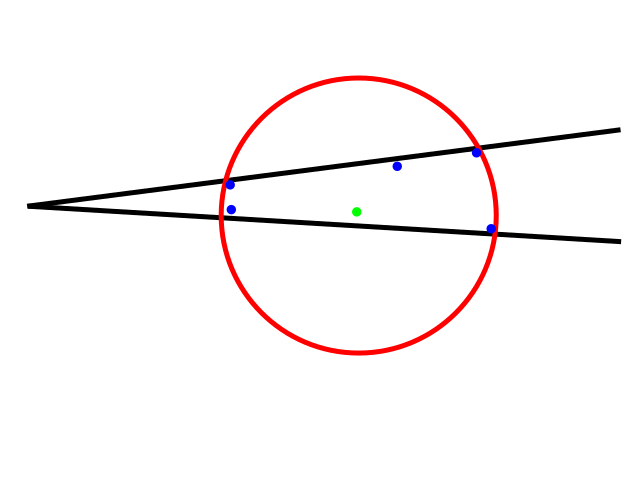
\includegraphics[scale=0.4]{images/bad_lambda.png}
    \caption[An example of constraints limiting sample point choices.]
    	{An example of constraints limiting sample point choices.   If the constraints remove a large region of the trust region, there may be no feasible $\Lambda$-poised set.
    }
    \label{lspc}
\end{figure}

%As the number of dimensions grows the ratio of volume of the trust region intersect the feasible region to the feasible region can become smaller.

One way to handle this is to  introduce a $\xi_{\text{cur}}$ which is allowed to decrease.
(Possibly, until a threshold is reached for maintaining a fixed $\Lambda$.)
If the new point does not improve the geometry of the set significantly, then there is no other point that would do better.
To test this, we introduce a constant $\delta_{\text{improv}}>0$ and require a new point to increase the current pivot by a factor greater than $\delta_{\text{improv}}$.
If the new point does not satisfy this test, we proceed with our current point and possibly decrease $\xi_{\text{cur}}$.
The new modified improvement algorithm is described in \cref{modified_model_improving_algorithm}:

\sbnote{We need to replace the following algorithm with the version that uses the pivot polynomials $u_i$ instead of $\phi_i$.}

\begin{algorithm}[H]
    \caption{Modified Model Improvement Algorithm}
    \label{modified_model_improving_algorithm}
    \begin{itemize}
        \item[\textbf{Step 0}] \textbf{(Initialization)} \\
            Initialize $i=1$.
            If the current sample set does not have $p$ points, repeat one of the current points. 
            Construct the Vandermonde matrix $V_{i,j} = \phi_j(\frac 1 {\Delta}(y^i - y^0))$.
            Initialize $0 < \ximin < \xi_{\text{desired}}$, $0 <\delta_{\text{improv}} < 1$,
            $  \xi_{\text{cur}} = \xi_{\text{desired}}$.
            
        \item[\textbf{Step 1}] \textbf{(Pivot)} \\
            Swap row $i$ with row $i_{\max} = \arg \max_{j|j\ge i} V_{j,i} $
        
        \item[\textbf{Step 2}] \textbf{(Check threshold)} \begin{itemize}
                \item[] If $|V_{i,i}| \ge \xi_{\text{cur}} $ then go to Step 3
                \item[] $ \hat y = \arg\max_{t \in \sampletrk \cap X} |\phi_i(t)|$
                \item[] If $\label{impossibly_poised} |\phi_i(\hat y)| < \ximin$ then \textbf{Stop}: the algorithm failed
                \item[] If $\xi_{\text{cur}} - |\phi_i(\hat y)| > \delta_{\text{improv}} \xi_{\text{cur}}$ then replace $V_{i,j}$ with $\phi_j(\hat y)$ and $\xi_{\text{cur}} \gets |\phi_i(\hat y)|$
            \end{itemize}
        
        \item[\textbf{Step 3}] \textbf{(LU)} \begin{itemize}
                \item[] Set $V_i \gets \frac{1}{V_{i,i}} V_i$
                \item[] Set $V_{,j} \gets V_{, j} - V_{i,j} V_{\bullet, i} \forall j=i \ldots p$
            \end{itemize}
            $i \gets i+1$
            Go to step 1 unless $i > p$
    \end{itemize}
\end{algorithm}

The \emph{ConstructTrustRegion} subroutine for this approach follows the prototype with $\sampletrk = \searchtrk = \feasible \cap \outertrk $.
As is usual, we may also wish to remove points larger than a certain radius from the current model center.
% If a lower bound $\kappa_{\phi}$ on the maximum value of each polynomial is known ahead of time, then the check on \cref{impossibly_poised} is not needed.
% That is, for a given set of linear constraints and largest trust region radius, it may be possible to calculate $\xi_{\text{min}} \le \kappa_{\phi} \le \max_{V}\max_{j}\max_{i}\|\phi_i(y^j)\|$.

%Another interesting approach we have not investigated is to decrease the size of the sample set when a new point cannot be computed.

%The analysis for this approach may be more difficult.






\newpage


\section{Results}


\subsection{Sample Problem}
The first test was on a problem with simple constraints and a pathological objective.
We let $f(x) = \epsilon x + (1-\epsilon)(y - \alpha x \sin(\gamma x))^2$ for a fixed constant $\epsilon$, and set the constraints to be
$x_2 \le ax_1$, $x_2 \ge -ax_1$ for a fixed constant $a$.

We summarize the number of function evaluations and iterations taken here:
\tiny
\begin{center}
\begin{longtable}{ c c c c c c c c }
Shape & Search & Num. Segments & Basis & Iterations & Evaluations \\
\hline
                spherical &   anywhere &       &     linear & 159  &   202  &  470 &  630 \\
                spherical &   anywhere &       &  quadratic & 164  &   277  &  467 &  805 \\
                spherical &       none &       &     linear &  77* &   122* &  255 &  387 \\
                spherical &       none &       &  quadratic &  74  &   149  &  250 &  561 \\
                spherical &    segment &     1 &     linear &  74  &   116  &  224 &  413 \\
                spherical &    segment &     1 &  quadratic &  74  &   164  &  224 &  525 \\
                spherical &    segment &     2 &     linear & 164  &   223  &  313 &  503 \\
                spherical &    segment &     2 &  quadratic & 152  &   259  &  313 &  657 \\
  circumscribed ellipsoid &       none &       &     linear &  41  &    50  &   41 &   55 \\
  circumscribed ellipsoid &       none &       &  quadratic &  41  &   104  &   41 &  105 \\
                ellipsoid &   anywhere &       &     linear &  65  &   109  &   67 &  110 \\
                ellipsoid &   anywhere &       &  quadratic &  66  &   170  &   67 &  185 \\
%                ellipsoid &  anywhere* &       &  quadratic &  61  &   157  &   60 &  155 \\
                ellipsoid &       none &       &     linear &  53  &    65  &   50 &   52 \\
                ellipsoid &       none &       &  quadratic &  53  &    88  &   50 &   75 \\
                ellipsoid &    segment &     1 &     linear &  55  &    70  &   58 &   75 \\
                ellipsoid &    segment &     1 &  quadratic &  55  &    97  &   58 &  104 \\
                ellipsoid &    segment &     2 &     linear &  67  &   144  &   68 &  121 \\
                ellipsoid &    segment &     2 &  quadratic &  67  &   196  &   64 &  159 \\
               polyhedral &       none &       &     linear &  37  &    43  &   38 &   46 \\
               polyhedral &       none &       &  quadratic &  37  &    82  &   38 &   89 \\
         scaled ellipsoid &   anywhere &       &     linear &  66  &   103  &   67 &  104 \\
         scaled ellipsoid &   anywhere &       &  quadratic &  68  &   156  &   67 &  169 \\
         scaled ellipsoid &    segment &     1 &     linear &  44  &    65  &   45 &   67 \\
         scaled ellipsoid &    segment &     1 &  quadratic &  44  &    94  &   45 &   93 \\
         scaled ellipsoid &    segment &     2 &     linear &  67  &   125  &   68 &  122 \\
         scaled ellipsoid &    segment &     2 &  quadratic &  67  &   189  &   63 &  146 \\
                  simplex & max volume &       &     linear &  41  &    44  &   41 &   45 \\
                  simplex & max volume &       &  quadratic &  41  &    94  &   41 &   84 \\

%                spherical &   anywhere &       &     linear &   159 &   202 \\
%                spherical &   anywhere &       &  quadratic &   164 &   277 \\
%                spherical &       none &       &     linear &    77* &   122* \\
%                spherical &       none &       &  quadratic &    74 &   149 \\
%                spherical &    segment &     1 &     linear &    74 &   116 \\
%                spherical &    segment &     1 &  quadratic &    74 &   164 \\
%                spherical &    segment &     2 &     linear &   164 &   223 \\
%                spherical &    segment &     2 &  quadratic &   152 &   259 \\
%  circumscribed ellipsoid &       none &       &     linear &    41 &    50 \\
%  circumscribed ellipsoid &       none &       &  quadratic &    41 &   104 \\
%                ellipsoid &   anywhere &       &     linear &    65 &   109 \\
%                ellipsoid &   anywhere &       &  quadratic &    66 &   170 \\
%                ellipsoid &  anywhere* &       &  quadratic &    61 &   157 \\
%                ellipsoid &       none &       &     linear &    53 &    65 \\
%                ellipsoid &       none &       &  quadratic &    53 &    88 \\
%                ellipsoid &    segment &     1 &     linear &    55 &    70 \\
%                ellipsoid &    segment &     1 &  quadratic &    55 &    97 \\
%                ellipsoid &    segment &     2 &     linear &    67 &   144 \\
%                ellipsoid &    segment &     2 &  quadratic &    67 &   196 \\
%               polyhedral &       none &       &     linear &    37 &    43 \\
%               polyhedral &       none &       &  quadratic &    37 &    82 \\
%         scaled ellipsoid &   anywhere &       &     linear &    66 &   103 \\
%         scaled ellipsoid &   anywhere &       &  quadratic &    68 &   156 \\
%         scaled ellipsoid &    segment &     1 &     linear &    44 &    65 \\
%         scaled ellipsoid &    segment &     1 &  quadratic &    44 &    94 \\
%         scaled ellipsoid &    segment &     2 &     linear &    67 &   125 \\
%         scaled ellipsoid &    segment &     2 &  quadratic &    67 &   189 \\
%                  simplex & max volume &       &     linear &    41 &    44 \\
%                  simplex & max volume &       &  quadratic &    41 &    94 \\

\end{longtable}
\end{center}
\normalsize

*The spherical trust region with no search for the center did not converge.

In general, the linear models converge more quickly than quadratic models.
We see that the method with fewest iterations and function evaluations is the linear polyhedral shape.
This is likely due to the fact that the polyhedral shape is allowed to search the entire outer trust region.
This also explains why the circumscribed ellipse and maximum volume simplex also perform well.
%We also notices that with a simple heuristic we were able to improve the ellipse slightly from 170 to 157.
Also, the scaled ellipsoid performs comparably to the unscaled version.

\subsection{Schittkowksi Test Problems}


We tested these algorithms on several problems from the Hot-Schittkowski problem set \cite{Schittkowski:1987:MTE:27135}, \cite{Hock1980}.
We selected the problems that have linear constraints: 21, 24, 25, 35, 36, 44, 45, 76, 224, 231, 232, 250, 251.

% 37 was left out because it proved to be difficult.

We summarize the results here.
\begin{tiny}

\begin{center}
\begin{longtable}{ c c c c c c c c c c }
Algorithm & Prob. & n & Message & N. It. & N. Eval. & Ret. Min. & Min. & Solution & Minimizer \\
\hline
  circumscribed ellipse   &   21  &  2  & converged  &   24  &   71  &  -99.960   &  -99.960   & [2.00,0.00] & [2.00,0.00] \\
         ellipse          &   21  &  2  & converged  &   36  &   96  &  -99.960   &  -99.960   & [2.00,0.00] & [2.00,0.00] \\
    ellipse everywhere    &   21  &  2  & converged  &   24  &   82  &  -99.960   &  -99.960   & [2.00,0.00] & [2.00,0.00] \\
    ellipse segment 1     &   21  &  2  & converged  &   24  &   84  &  -99.960   &  -99.960   & [2.00,0.00] & [2.00,0.00] \\
    ellipse segment 2     &   21  &  2  & converged  &   24  &   85  &  -99.960   &  -99.960   & [2.00,0.00] & [2.00,0.00] \\
        polyhedral        &   21  &  2  & converged  &   26  &   75  &  -99.960   &  -99.960   & [2.00,-0.00] & [2.00,0.00] \\
  circumscribed ellipse   &  224  &  2  &   failed   &   16  &   56  &  -304.000  &  -304.000  & [4.00,4.00] & [4.00,4.00] \\
         ellipse          &  224  &  2  & converged  &   32  &   97  &  -304.000  &  -304.000  & [4.00,4.00] & [4.00,4.00] \\
    ellipse everywhere    &  224  &  2  & converged  &   24  &   94  &  -303.774  &  -304.000  & [3.73,4.27] & [4.00,4.00] \\
    ellipse segment 1     &  224  &  2  & converged  &   24  &   91  &  -303.774  &  -304.000  & [3.73,4.27] & [4.00,4.00] \\
    ellipse segment 2     &  224  &  2  & converged  &   23  &   89  &  -303.774  &  -304.000  & [3.73,4.27] & [4.00,4.00] \\
        polyhedral        &  224  &  2  & converged  &   17  &   64  &  -304.000  &  -304.000  & [4.00,4.00] & [4.00,4.00] \\
  circumscribed ellipse   &  231  &  2  & converged  &   14  &   44  &   0.000    &   0.000    & [1.00,1.00] & [1.00,1.00] \\
         ellipse          &  231  &  2  & converged  &   99  &  193  &   0.000    &   0.000    & [1.00,1.00] & [1.00,1.00] \\
    ellipse everywhere    &  231  &  2  & converged  &  181  &  336  &   0.000    &   0.000    & [1.00,1.00] & [1.00,1.00] \\
    ellipse segment 1     &  231  &  2  & converged  &   78  &  162  &   0.000    &   0.000    & [1.00,1.00] & [1.00,1.00] \\
    ellipse segment 2     &  231  &  2  & converged  &  173  &  321  &   0.000    &   0.000    & [1.00,1.00] & [1.00,1.00] \\
        polyhedral        &  231  &  2  & converged  &   95  &  193  &   0.000    &   0.000    & [1.00,1.00] & [1.00,1.00] \\
  circumscribed ellipse   &  232  &  2  &   failed   &   15  &   35  &   -1.000   &   -1.000   & [3.00,1.73] & [3.00,1.73] \\
         ellipse          &  232  &  2  & converged  &   34  &   91  &   -1.000   &   -1.000   & [3.00,1.73] & [3.00,1.73] \\
    ellipse everywhere    &  232  &  2  & converged  &   41  &  102  &   -1.000   &   -1.000   & [3.00,1.73] & [3.00,1.73] \\
    ellipse segment 1     &  232  &  2  & converged  &   34  &   91  &   -1.000   &   -1.000   & [3.00,1.73] & [3.00,1.73] \\
    ellipse segment 2     &  232  &  2  & converged  &   35  &   95  &   -1.000   &   -1.000   & [3.00,1.73] & [3.00,1.73] \\
        polyhedral        &  232  &  2  & converged  &   15  &   47  &   -1.000   &   -1.000   & [3.00,1.73] & [3.00,1.73] \\
  circumscribed ellipse   &   24  &  2  &   failed   &   15  &   35  &   -1.000   &   -1.000   & [3.00,1.73] & [3.00,1.73] \\
         ellipse          &   24  &  2  & converged  &   34  &   90  &   -1.000   &   -1.000   & [3.00,1.73] & [3.00,1.73] \\
    ellipse everywhere    &   24  &  2  & converged  &   41  &  104  &   -1.000   &   -1.000   & [3.00,1.73] & [3.00,1.73] \\
    ellipse segment 1     &   24  &  2  & converged  &   34  &   91  &   -1.000   &   -1.000   & [3.00,1.73] & [3.00,1.73] \\
    ellipse segment 2     &   24  &  2  & converged  &   35  &   95  &   -1.000   &   -1.000   & [3.00,1.73] & [3.00,1.73] \\
        polyhedral        &   24  &  2  & converged  &   15  &   47  &   -1.000   &   -1.000   & [3.00,1.73] & [3.00,1.73] \\
  circumscribed ellipse   &  250  &  3  &   failed   &   24  &  103  & -3300.000  & -3300.000  & [20.00,11.00,15.00] & [20.00,11.00,15.00] \\
         ellipse          &  250  &  3  & converged  &   53  &  207  & -3300.000  & -3300.000  & [20.00,11.00,15.00] & [20.00,11.00,15.00] \\
    ellipse everywhere    &  250  &  3  &   failed   &   48  &  103  & -3298.196  & -3300.000  & [19.99,10.99,15.02] & [20.00,11.00,15.00] \\
    ellipse segment 1     &  250  &  3  &   failed   &   53  &  112  & -3299.243  & -3300.000  & [19.99,11.00,15.01] & [20.00,11.00,15.00] \\
    ellipse segment 2     &  250  &  3  &   failed   &   54  &  112  & -3299.082  & -3300.000  & [19.99,11.00,15.01] & [20.00,11.00,15.00] \\
    ellipse segment 3     &  250  &  3  &   failed   &   56  &  116  & -3299.504  & -3300.000  & [19.99,11.00,15.00] & [20.00,11.00,15.00] \\
        polyhedral        &  250  &  3  & converged  &   26  &  113  & -3300.000  & -3300.000  & [20.00,11.00,15.00] & [20.00,11.00,15.00] \\
  circumscribed ellipse   &  251  &  3  &   failed   &   20  &   86  & -3456.000  & -3456.000  & [24.00,12.00,12.00] & [24.00,12.00,12.00] \\
         ellipse          &  251  &  3  &   failed   &   10  &   53  & -3454.018  & -3456.000  & [23.55,12.06,12.16] & [24.00,12.00,12.00] \\
    ellipse everywhere    &  251  &  3  &   failed   &   6   &   17  & -3209.710  & -3456.000  & [22.82,13.03,10.79] & [24.00,12.00,12.00] \\
    ellipse segment 1     &  251  &  3  &   failed   &   4   &   13  & -1698.807  & -3456.000  & [21.71,9.21,8.50] & [24.00,12.00,12.00] \\
    ellipse segment 2     &  251  &  3  &   failed   &   6   &   17  & -3210.341  & -3456.000  & [21.49,11.46,13.04] & [24.00,12.00,12.00] \\
    ellipse segment 3     &  251  &  3  &   failed   &   14  &   64  & -3449.803  & -3456.000  & [22.84,12.29,12.29] & [24.00,12.00,12.00] \\
        polyhedral        &  251  &  3  & converged  &   22  &  124  & -3456.000  & -3456.000  & [24.00,12.00,12.00] & [24.00,12.00,12.00] \\
  circumscribed ellipse   &   25  &  3  & converged  &  760  &  1472 &   0.000    &   0.000    & [52.92,24.90,1.52] & [50.00,25.00,1.50] \\
    ellipse everywhere    &   25  &  3  &   failed   &   1   &   1   &   32.835   &   0.000    & [100.00,12.50,3.00] & [50.00,25.00,1.50] \\
    ellipse segment 1     &   25  &  3  &   failed   &   1   &   1   &   32.835   &   0.000    & [100.00,12.50,3.00] & [50.00,25.00,1.50] \\
    ellipse segment 2     &   25  &  3  &   failed   &   1   &   1   &   32.835   &   0.000    & [100.00,12.50,3.00] & [50.00,25.00,1.50] \\
    ellipse segment 3     &   25  &  3  &   failed   &   1   &   1   &   32.835   &   0.000    & [100.00,12.50,3.00] & [50.00,25.00,1.50] \\
        polyhedral        &   25  &  3  & converged  &  1793 &  3396 &   0.000    &   0.000    & [50.94,24.97,1.51] & [50.00,25.00,1.50] \\
  circumscribed ellipse   &   35  &  3  &   failed   &  781  &  1028 &   0.111    &   0.111    & [1.33,0.78,0.44] & [1.33,0.78,0.44] \\
         ellipse          &   35  &  3  & converged  &   28  &  122  &   0.111    &   0.111    & [1.33,0.78,0.44] & [1.33,0.78,0.44] \\
    ellipse everywhere    &   35  &  3  &   failed   &   24  &   82  &   0.113    &   0.111    & [1.36,0.79,0.42] & [1.33,0.78,0.44] \\
    ellipse segment 1     &   35  &  3  &   failed   &   16  &   76  &   0.112    &   0.111    & [1.31,0.79,0.45] & [1.33,0.78,0.44] \\
    ellipse segment 2     &   35  &  3  &   failed   &   16  &   75  &   0.112    &   0.111    & [1.31,0.79,0.45] & [1.33,0.78,0.44] \\
    ellipse segment 3     &   35  &  3  &   failed   &   16  &   77  &   0.112    &   0.111    & [1.31,0.79,0.45] & [1.33,0.78,0.44] \\
        polyhedral        &   35  &  3  & converged  &   14  &  112  &   0.111    &   0.111    & [1.33,0.78,0.44] & [1.33,0.78,0.44] \\
  circumscribed ellipse   &   36  &  3  &   failed   &   19  &   81  & -3300.000  & -3300.000  & [20.00,11.00,15.00] & [20.00,11.00,15.00] \\
         ellipse          &   36  &  3  & converged  &   53  &  202  & -3300.000  & -3300.000  & [20.00,11.00,15.00] & [20.00,11.00,15.00] \\
    ellipse everywhere    &   36  &  3  &   failed   &   63  &  135  & -3299.808  & -3300.000  & [20.00,11.00,15.00] & [20.00,11.00,15.00] \\
    ellipse segment 1     &   36  &  3  &   failed   &   64  &  140  & -3299.951  & -3300.000  & [20.00,11.00,15.00] & [20.00,11.00,15.00] \\
    ellipse segment 2     &   36  &  3  &   failed   &   64  &  133  & -3299.918  & -3300.000  & [20.00,11.00,15.00] & [20.00,11.00,15.00] \\
    ellipse segment 3     &   36  &  3  &   failed   &   65  &  137  & -3299.870  & -3300.000  & [20.00,11.00,15.00] & [20.00,11.00,15.00] \\
        polyhedral        &   36  &  3  & converged  &   22  &  108  & -3300.000  & -3300.000  & [20.00,11.00,15.00] & [20.00,11.00,15.00] \\
  circumscribed ellipse   &   37  &  3  &   failed   &   27  &   98  & -3456.000  & -3456.000  & [24.00,12.00,12.00] & [24.00,12.00,12.00] \\
         ellipse          &   37  &  3  &   failed   &   15  &   65  & -3455.761  & -3456.000  & [23.94,12.01,12.02] & [24.00,12.00,12.00] \\
    ellipse everywhere    &   37  &  3  &   failed   &   36  &   88  & -3406.653  & -3456.000  & [27.34,10.93,11.40] & [24.00,12.00,12.00] \\
    ellipse segment 1     &   37  &  3  &   failed   &   30  &   82  & -3421.619  & -3456.000  & [21.29,12.62,12.73] & [24.00,12.00,12.00] \\
    ellipse segment 2     &   37  &  3  &   failed   &   36  &   85  & -3415.110  & -3456.000  & [21.05,12.70,12.78] & [24.00,12.00,12.00] \\
    ellipse segment 3     &   37  &  3  &   failed   &   28  &   75  & -3421.157  & -3456.000  & [21.31,12.55,12.79] & [24.00,12.00,12.00] \\
        polyhedral        &   37  &  3  & converged  &   28  &  139  & -3456.000  & -3456.000  & [24.00,12.00,12.00] & [24.00,12.00,12.00] \\
  circumscribed ellipse   &   44  &  4  &   failed   &   17  &  124  &  -13.000   &  -15.000   & [3.00,-0.00,4.00,0.00] & [0.00,3.00,0.00,4.00] \\
         ellipse          &   44  &  4  & converged  &   50  &  298  &  -15.000   &  -15.000   & [0.00,3.00,-0.00,4.00] & [0.00,3.00,0.00,4.00] \\
    ellipse everywhere    &   44  &  4  & converged  &  110  &  416  &  -15.000   &  -15.000   & [0.00,3.00,0.00,4.00] & [0.00,3.00,0.00,4.00] \\
    ellipse segment 1     &   44  &  4  & converged  &   50  &  262  &  -15.000   &  -15.000   & [-0.00,3.00,0.00,4.00] & [0.00,3.00,0.00,4.00] \\
    ellipse segment 2     &   44  &  4  & converged  &   71  &  304  &  -15.000   &  -15.000   & [-0.00,3.00,0.00,4.00] & [0.00,3.00,0.00,4.00] \\
    ellipse segment 3     &   44  &  4  &   failed   &   7   &   32  &  -10.672   &  -15.000   & [-0.00,2.55,0.36,3.41] & [0.00,3.00,0.00,4.00] \\
    ellipse segment 4     &   44  &  4  &   failed   &   1   &   1   &   -1.338   &  -15.000   & [1.44,0.98,1.80,1.80] & [0.00,3.00,0.00,4.00] \\
        polyhedral        &   44  &  4  & converged  &   15  &  134  &  -13.000   &  -15.000   & [3.00,-0.00,4.00,-0.00] & [0.00,3.00,0.00,4.00] \\
  circumscribed ellipse   &   45  &  5  &   failed   &   21  &  190  &   1.000    &   1.000    & [1.00,2.00,3.00,4.00,5.00] & [1.00,2.00,3.00,4.00,5.00] \\
         ellipse          &   45  &  5  & converged  &   51  &  405  &   1.000    &   1.000    & [1.00,2.00,3.00,4.00,5.00] & [1.00,2.00,3.00,4.00,5.00] \\
    ellipse everywhere    &   45  &  5  & converged  &  414  &  1121 &   1.000    &   1.000    & [1.00,2.00,3.00,4.00,5.00] & [1.00,2.00,3.00,4.00,5.00] \\
    ellipse segment 1     &   45  &  5  & converged  &   63  &  374  &   1.000    &   1.000    & [1.00,2.00,3.00,4.00,5.00] & [1.00,2.00,3.00,4.00,5.00] \\
    ellipse segment 2     &   45  &  5  & converged  &   82  &  404  &   1.000    &   1.000    & [1.00,2.00,3.00,4.00,5.00] & [1.00,2.00,3.00,4.00,5.00] \\
    ellipse segment 3     &   45  &  5  & converged  &  104  &  453  &   1.000    &   1.000    & [1.00,2.00,3.00,4.00,5.00] & [1.00,2.00,3.00,4.00,5.00] \\
    ellipse segment 4     &   45  &  5  & converged  &  130  &  497  &   1.000    &   1.000    & [1.00,2.00,3.00,4.00,5.00] & [1.00,2.00,3.00,4.00,5.00] \\
    ellipse segment 5     &   45  &  5  & converged  &  158  &  478  &   1.000    &   1.000    & [1.00,2.00,3.00,4.00,5.00] & [1.00,2.00,3.00,4.00,5.00] \\
        polyhedral        &   45  &  5  & converged  &   22  &  269  &   1.000    &   1.000    & [1.00,2.00,3.00,4.00,5.00] & [1.00,2.00,3.00,4.00,5.00] \\
  circumscribed ellipse   &   76  &  4  &   failed   &   15  &  111  &   -4.682   &   -4.682   & [0.27,2.09,-0.00,0.55] & [0.27,2.09,-0.00,0.55] \\
         ellipse          &   76  &  4  &   failed   &   17  &  137  &   -4.682   &   -4.682   & [0.27,2.09,0.00,0.54] & [0.27,2.09,-0.00,0.55] \\
    ellipse everywhere    &   76  &  4  &   failed   &   25  &  106  &   -4.604   &   -4.682   & [0.45,1.89,-0.00,0.77] & [0.27,2.09,-0.00,0.55] \\
    ellipse segment 1     &   76  &  4  &   failed   &   17  &  111  &   -4.682   &   -4.682   & [0.27,2.09,-0.00,0.54] & [0.27,2.09,-0.00,0.55] \\
    ellipse segment 2     &   76  &  4  &   failed   &   24  &  105  &   -4.680   &   -4.682   & [0.31,2.08,0.00,0.52] & [0.27,2.09,-0.00,0.55] \\
    ellipse segment 3     &   76  &  4  &   failed   &   25  &  106  &   -4.677   &   -4.682   & [0.34,2.07,0.00,0.51] & [0.27,2.09,-0.00,0.55] \\
    ellipse segment 4     &   76  &  4  &   failed   &   23  &  107  &   -4.674   &   -4.682   & [0.34,2.03,-0.00,0.60] & [0.27,2.09,-0.00,0.55] \\
        polyhedral        &   76  &  4  & converged  &   15  &  169  &   -4.682   &   -4.682   & [0.27,2.09,-0.00,0.55] & [0.27,2.09,-0.00,0.55]
\end{longtable}
\end{center}


\end{tiny}

In order to better evaluate the algorithms on the problems across in this test set, we use a performance profile developed in \cite{More:2009:BDO:1654367.1654371}.
Given a set of Solvers $\mathcal S$ that solved a set of problems $\mathcal P$ with the number of evaluations of solver $s$ on problem $p$ being $N(s, p)$, the performance ratio is defined to be $r(s, p) = \frac{N(s, p)}{\min_{s \in \mathcal S} N(s, p)}$.
If the algorithm does not complete, then the number of evaluations is set to $\infty$.
The performance profile of a solver $s$ and parameter $\alpha \in [0, \infty)$ is then the number of problems for which the performance ratio is less than or equal to $\alpha$: 

\begin{align}
\rho(s, \alpha) = \frac 1 {\|\mathcal P \|} \|p \in \mathcal P | r(s, p) \le \alpha\|.
\end{align}

The $y$ axis of a performance plot is the performance profile, and the $x$ axis is the parameter $\alpha$.
Note that algorithms with high performance profiles for small values of $alpha$ solved a large number of problems the most with the fewest evaluations, while algorithms that eventually reach high performance profiles with larger values of $\alpha$ solve a large set of problems.
The performance profile for the Hot-Schittkowski problem set is give in figure \cref{performance_profile}.


\begin{figure}[ht]
    \centering
    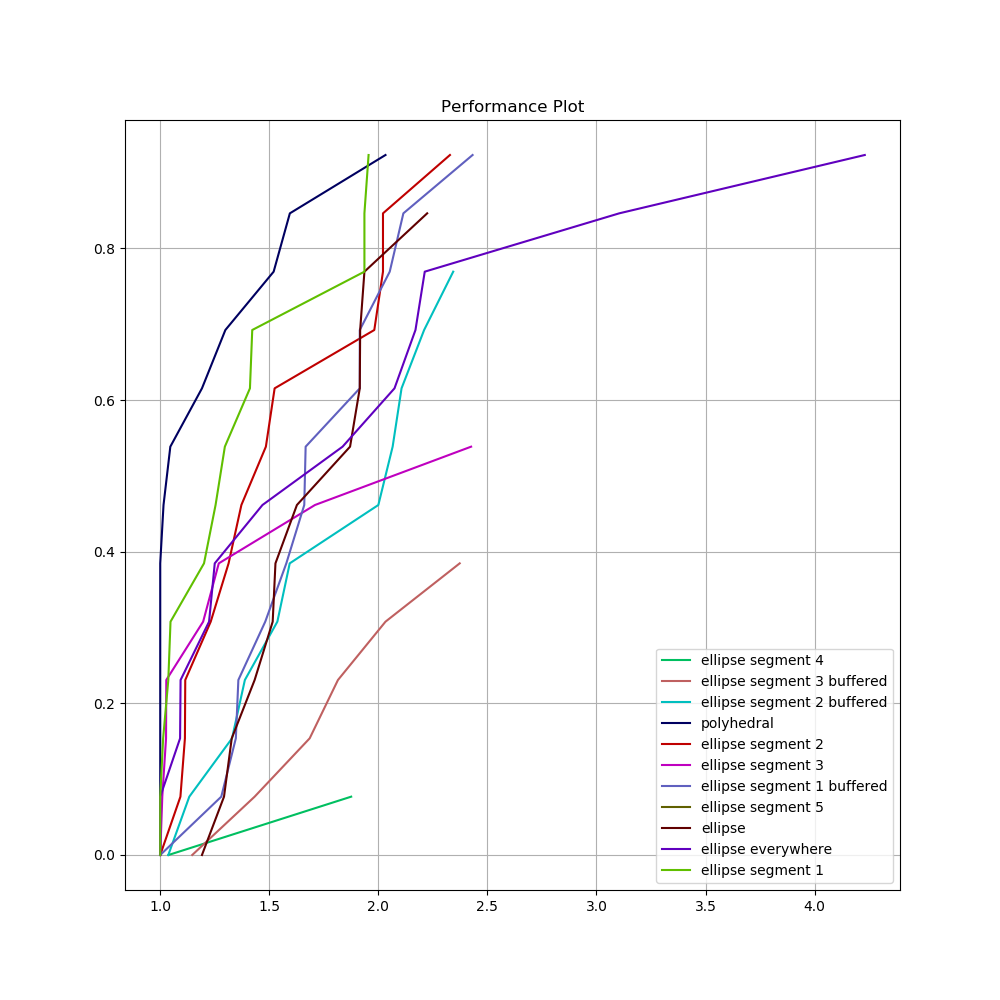
\includegraphics[scale=0.4]{images/performance_profile_plot.png}
    \caption{
    	\emph{Short:} A performance profile comparing different variants of the algorithm for linear constraints.
    	\emph{Long:} A performance profile comparing different variants of the algorithm for linear constraints.
    	We see that the polyhedral algorithm is both efficient and robust.
    }
    \label{performance_profile}
\end{figure}



The line segment search with 5 segments does not solve many problems, this is because several of the problems have dimension less than $5$, so that it was not even ran on these.
Notice that the polyhedral search does very well.
We conjecture that this may not hold with modelled, nonlinear constraints.


\subsection{Summary}
We still experienced a problem with iterates coming too close to the boundary of the feasible region.
Another way of dealing with this is to shift the constraints closer to the current iterate.
Namely, we introduce a parameter $\upsilon$ to determine how far to scale the constraints.
Then, within the trust region subproblem, we add constraints of $Ax \le b\upsilon + (1-\upsilon) A \xk $.
Before doing this, the rows of $A$ are normalized.
This produces the buffered segment searches withing the results.

% \color{red}
% 
% \section{Figure out where goes}
% 
% From here on, we will assume that the iterates $\xk$ are chosen according to \cref{linearly_constrained_dfo}.
% This implies that each of the sample points used to construct $\mfk$ are output of \cref{model_improving_algorithm}.
% 
% Because \cref{lipschitz_gradient} and \cref{lipschitz_hessian} are satisfied, $f$ also satisfies \cref{introduction_3_1} and hence the assumptions for \cref{quadratic_errors}.
% Notice that because $\kappa_f$, $\kappa_g$, $\kappa_h$ only depend on $p$, $L_h$, and $\Lambda$, these values do not depend on the iteration $k$:
% using the same tolerance $\xi_{\text{min}}$ within \cref{model_improving_algorithm} implies a bound on $\Lambda$.
% , and therefore $\mfk$ satisfies the requirements for \cref{quadratic_errors}.
% is a fully quadratic model over $B_{\infty}(\xk, \dk)$.
% \color{black}

\section{Deleted Stuff}


\section{Ellipsoidal Trust Region Approach}

If we adopt the ellipsoidal trust region approach to maintain a feasible inner trust region with a ``nice" shape we ensure of a stronger version of \cref{accuracy}.
Namely, we know from \cref{ellipsoidal_lambda} that 
\begin{align*}
    \|\mfk(x) - \nabla f(x) \| \le \kappa_g \Delta_{k} \quad \forall x \in \searchtrk.
\end{align*}
If we also choose our trial point with \cref{search_a_little}, we have no guarantee of satisfying the efficiency condition \cref{efficiency} because $\dk$ is the outer trust region radius.
However, the model will likely be more accurate over this region.

%If bounds can be shown relating the model error of the inner trust region to the outer trust region, then we will satisfy \cref{accuracy}.
%In this case, classical methods ensure that $\|\nabla f(x^{(k)}) - \nabla m_f(x^{(k)})\| < \Delta_{inner} \le \dk$.


\subsection{Ellipsoid Choices}

In order to address this issue we considered using ellipsoidal trust regions.
Whereas the circle does not allow improvement when the current iterate lies along a constraint, an ellipsoid elongates along this constraint.
In figure \cref{ellipse_adv}, we have this type of iterate, but by using an ellipsoid we are still able to search towards the vertex of the feasible region.
\begin{figure}[ht]
    \centering
    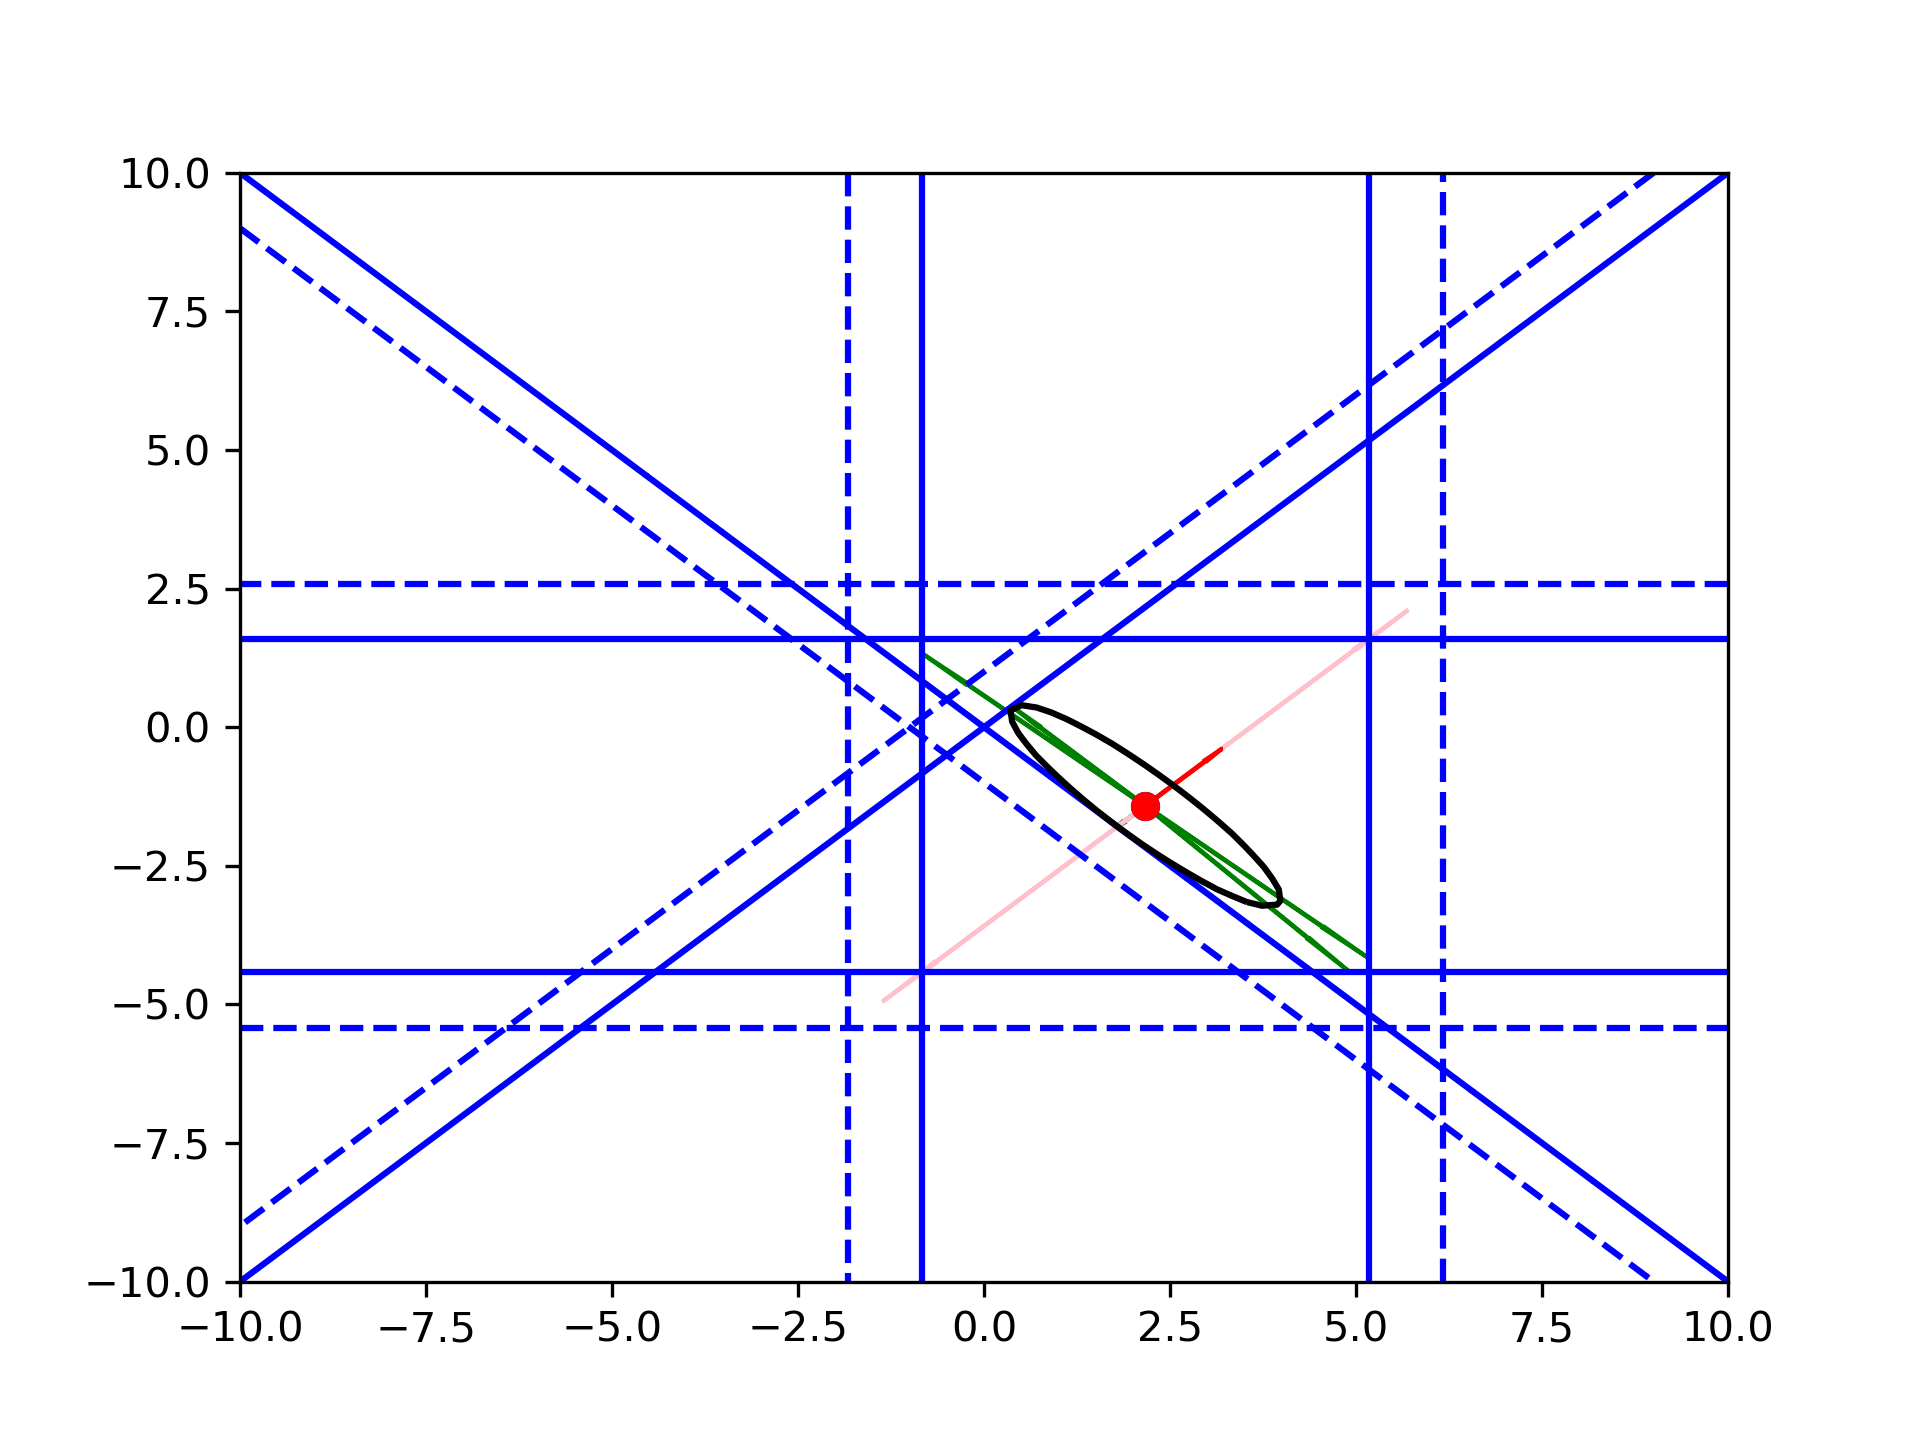
\includegraphics[scale=0.4]{images/advantage_of_ellipse_2.png}
    \caption{
    	\emph{Short:} An ellipsoidal trust region allows for more progress than a circular trust region.
    	\emph{Long:} Although the center of the ellipsoid is close to the boundary of the constraints, it can elongate to allow progress.
    }
    \label{ellipse_adv}
\end{figure}


More specifically, at iteration $k$, we choose a scaling factor $\sdk$ and solve for an ellipsoid center $\ck \in \Rn$ and positive definite matrix $\qk$ to define an ellipsoid
\begin{align*}
\ellipsek = \left\{x \in \Rn \bigg| \; \frac 1 2 \left(x - \ck\right)^T\qk\left(x - \ck\right) \le \frac 1 2 \sdk^2 \right\}.
\end{align*}
The simplest approach is to simply let the center of the ellipsoid be the current iterate: $\ck = \xk$.





\subsubsection{Ellipsoid Choices}

There are a number of issues to be solved to define this ellipsoid:
\begin{itemize}
\item How do we ensure that $\xk \in \ellipsek $?
\item How do we choose $\ellipsek$ in such a way that it does not limit travel along a decent direction?
\item How do we choose the center of the ellipsoid $\ck$?
\end{itemize}

% \item How do we choose $\ellipsek$ to make the  ellipsoid as large as possible while ensuring that $ \ellipsek \subset \outertrk \cap \feasible $?




\subsection{Circular Trust Region}
The simplest approach to maintaining a feasible trust region is to set the inner trust region radius sufficiently small.
Within the \emph{ConstructTrustRegion} subroutine, this method sets the trust region radius to the distance to the closest constraint:
$\outertrk = B_2\left(\xk, \min\left\{\dk, \min_{i}\frac{\left|A_i\xk - b_i\right|}{\left\|A_i\right\|} \right\}\right)$.
In practice, this does not work well as the radius can become too small to allow adequate progress.

Two general strategies were considered for addressing this issue as illustrated in \cref{options_basis}.
One option is to shift the center of the inner trust region as long as it remains within the outer trust region.
The second option is to elongate the trust region along the nearest constraint as discussed in the next section.
Of course, both of these can be done at the same time.


\begin{figure}[ht]
    \centering
    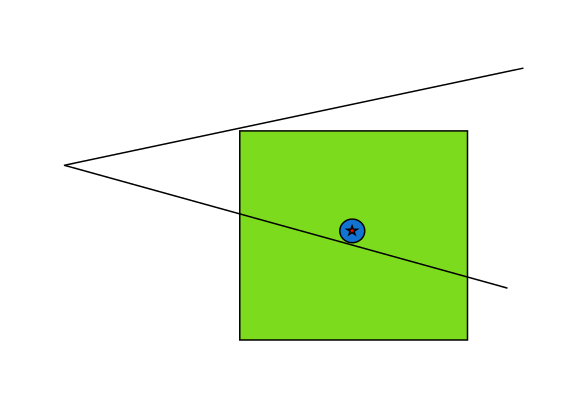
\includegraphics[width=200px]{images/small_circle.png}
    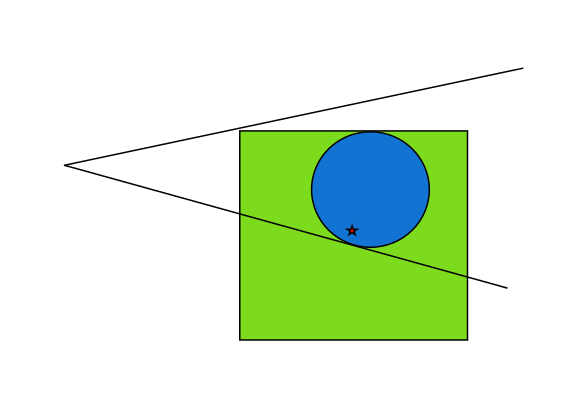
\includegraphics[width=200px]{images/shifted_center.png}
    \caption{
    	\emph{Short:} The advantage of not requiring the sample region center to be the trust region center.
    	\emph{Long:} When the current iterate is too close to a constraint, the circular trust region becomes too small.
    	Shifting the trust region center helps remedy this.
    	The star is the current iterate, the green is the outer trust region, and blue the inner.
    }
    \label{options_basis}
\end{figure}



====================


\sbnote{Move the following to somewhere else.}

The advantage of the ellipsoidal trust region approach \cref{bluepill} is that we can reuse classical methods for ensuring good geometry.
We can construct $\sampletrk$ to be ellipsoidal and use efficient algorithms within \cite{introduction_book} to satisfy \cref{accuracy}.
However, we must be careful while choosing $ \searchtrk$ to allow sufficient reduction when we solve the trust region subproblem using the inner trust region.
The search trust region is used while selecting the next iterate:
\begin{align*}
\sk = \argmin_{s \in \searchtrk} \mfk(\xk + s).
\end{align*}
=====================
